\documentclass[10pt,twocolumn,letterpaper]{article}

\usepackage{3dv2016authorkit/latex/3dv}
\usepackage{times}
\usepackage{epsfig}
\usepackage{graphicx}
\usepackage{amsmath}
\usepackage{amssymb}

% Include other packages here, before hyperref.
%\usepackage{multicol}
\usepackage{url}
\usepackage{subfigure}
\usepackage{graphicx}
\usepackage{caption}
\usepackage{array}
%\usepackage{arydshln}

% If you comment hyperref and then uncomment it, you should delete
% egpaper.aux before re-running latex.  (Or just hit 'q' on the first latex
% run, let it finish, and you should be clear).
%\usepackage[pagebackref=true,breaklinks=true,letterpaper=true,colorlinks,bookmarks=false]{hyperref}

%\threedvfinalcopy % *** Uncomment this line for the final submission

\def\threedvPaperID{4} % *** Enter the 3DV Paper ID here
\def\httilde{\mbox{\tt\raisebox{-.5ex}{\symbol{126}}}}

% Pages are numbered in submission mode, and unnumbered in camera-ready
\ifthreedvfinal\pagestyle{empty}\fi
\setcounter{page}{4321}
\begin{document}

%%%%%%%%% TITLE
\title{A Large-Scale 3D Object Recognition dataset}

\author{Thomas S{\o}lund\\
Danish Technological Institute\\
DK-5230 Odense M, Denmark\\
{\tt\small thso@dti.dk}
%For a paper whose authors are all at the same institution,
% omit the following lines up until the closing ``}''.
% Additional authors and addresses can be added with ``\and'',
% just like the second author.
% To save space, use either the email address or home page, not both
\and
Anders Glent Buch, Norbert Kr\"u{}ger\\
M\ae{}rsk Mc-Kinney M\o{}ller Institute,\\
University of Southern Denmark,\\
DK-5230 Odense, Denmark \\
{\tt\small anbu,norbert@mmmi.sdu.dk}
\and
Henrik Aan\ae s\\ %Knut Conradsen, 
Department of Applied Mathematics\\ and Computer Science,\\ 
Technical University of Denmark\\
DK-2800 Kgs. Lyngby, Denmark\\
{\tt\small aanes@dtu.dk} %knco,
}

\maketitle
%\thispagestyle{empty}

%%%%%%%%% ABSTRACT
\begin{abstract}
This paper presents a new large scale dataset targeting evaluation of local shape descriptors and 3d object recognition algorithms. The dataset consists of point clouds and triangulated meshes from 292 physical scenes take from 11 different views; a total of approximately 3200 views. Each of the physical scenes contain 10 occluded objects resulting in a dataset with around 32000 unique object poses and 45 different object models. The 45 object models are full 360 degree models which are scanned with a high precision structured light scanner and a turntable. All the included objects belongs to different geometric groups; concave, convex, cylindrical and flat 3D object models. The object models have varying amount of local geometric features to challenge existing local shape feature descriptors in terms of descriptiveness and robustness.  The dataset is validated in a benchmark which evaluates the matching performance of 7 different state-of-the-art local shape descriptors. Further, we validate the dataset in a 3D object recognition pipeline. Our benchmark shows as expected that local shape feature descriptors without any global point relation across the surface have a poor matching performance with flat and cylindrical objects. It is our objective that this dataset contributes to the future development of next generation of 3D object recognition algorithms. The dataset will be made public available.
\end{abstract}

%%%%%%%%% BODY TEXT

%%%%%%%%%%Page limits = 8 exclusive references
%Intro and related work -> 2.5 page
%Experiantal design -> 1 page
%Benchmark -> 1 page
%Evaluation/results -> 3 pages
% conclusion/discussion -> 1/2 page
\section{Introduction} %Hvad, hvorfor, hvordan
Object recognition in range images is a fundamental research area in computer vision with many different applications in different industries. With the continually introduction of new inexpensive 3D sensors for different applications, the ability to localize and recognize rigid and no rigid objects is an attractive and unavoidable technology. Applications areas such as robotic assembly, bin-picking, mobile robotic manipulation, biometric analysis, tracking and intelligent surveillance all benefits from 3D data for localizing objects. Mainly, because the third dimension is explicit given and not inferred as in 2D object pose estimation. In the last decades many contributions on 2D object recognition and classification have been published, where methods are evaluated on large-scale dataset like the PASCAL Visual Object Challenge (VOC) \cite{Everingham2014} and ImageNet \cite{Imagenet2009}. The benefit from evaluating algorithms on a large-scale dataset has proven valuable in the continues improvement of recognition algorithms after the release of the PASCAL VOC and ImageNet datasets \cite{Everingham2014}.
\begin{figure}[t]
\centering
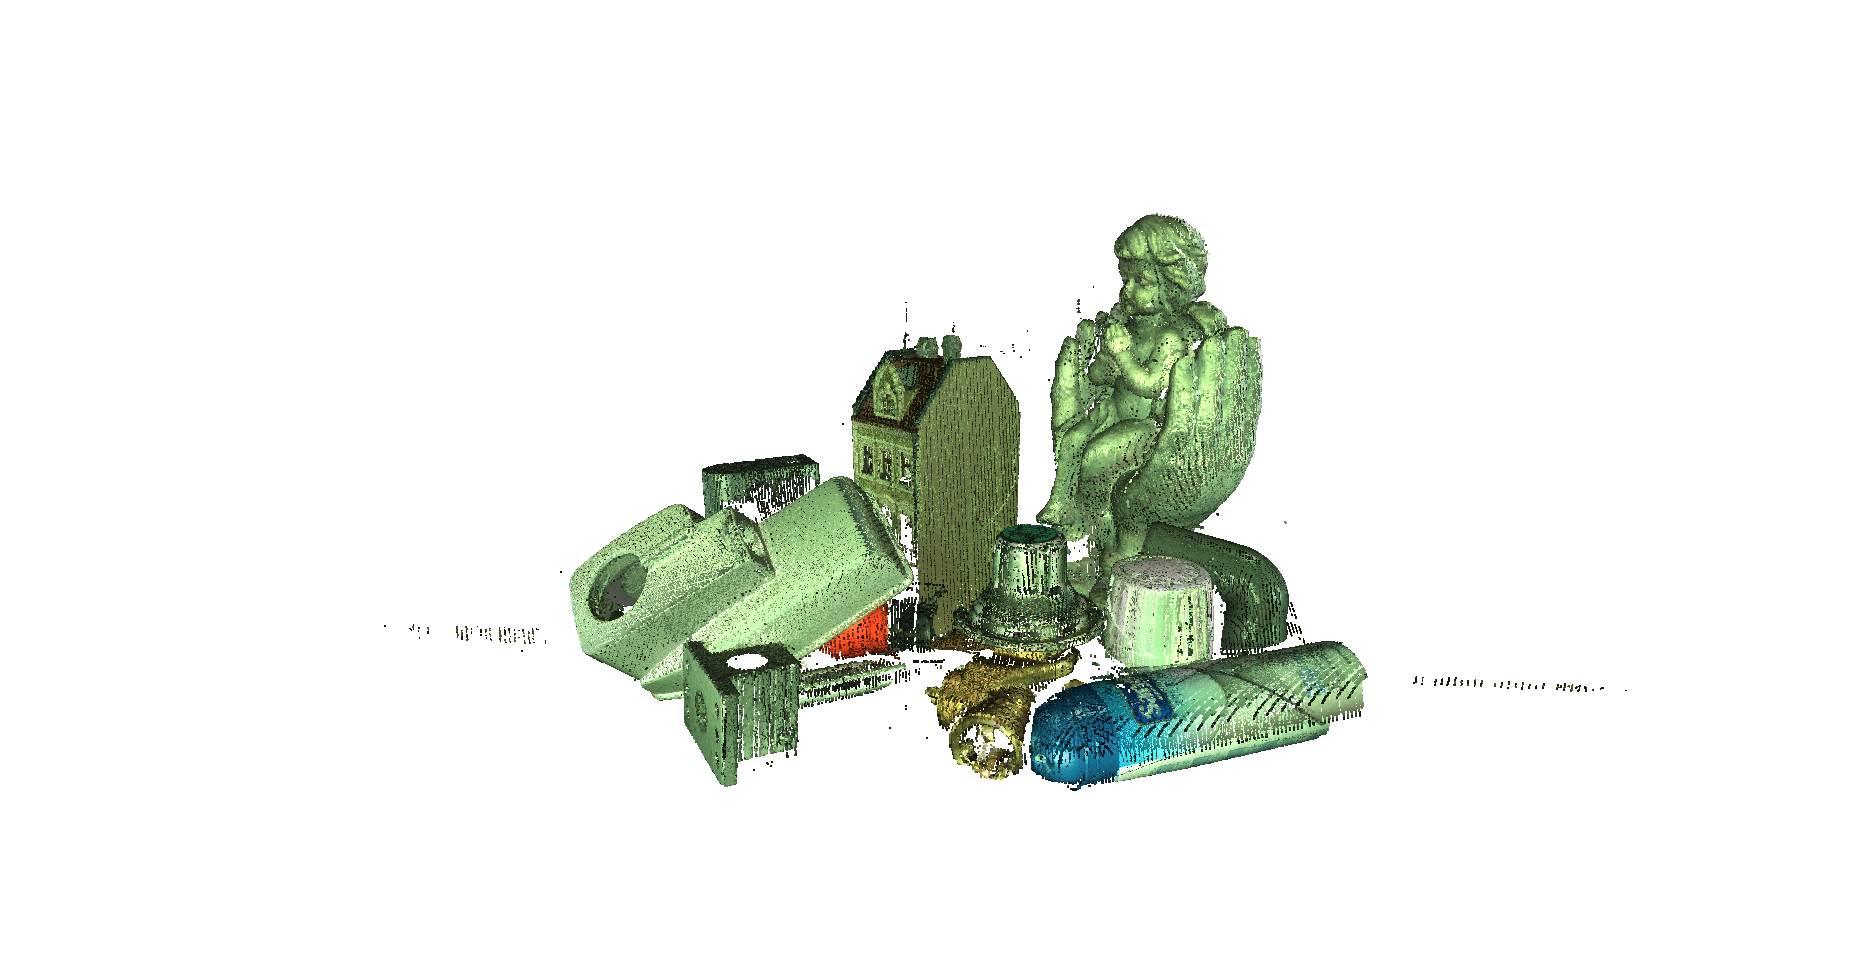
\includegraphics[clip, trim=14cm 5cm 10cm 5cm,width=0.8\linewidth, height= 0.8\linewidth, keepaspectratio]{img/scenes/full_scene00.png}
\caption{Example of a full registered scene included in the dataset}
\label{fig:scene}
\end{figure}
In 3D object recognition research, large-scale datasets that consist of a set of 3D querie models $Q_n$, 3D target scenes $S_t$ and ground truth poses $T_{gt}$ for each object in each scene are required in order to be able to evaluate existing and future 3D object recognition algorithms better. Until now, 3D object recognition algorithms are evaluated with eight smaller datasets \cite{Guo2015}, including in the UWA \cite{Mian2006},\cite{Mian2010}, Queens \cite{Taati2007},\cite{Taati2007} and Bologna \cite{Salti2014},\cite{Tombari2010} datasets. Other, smaller dataset like the Vienna Kinect\cite{Aldoma2012}, TUM \cite{Rodola2013}, TUM-LineMod\cite{Hinterstoisser2012}, BigBird\cite{BigBIRD} and RGB-D dataset version 1 \& 2 \cite{Lai2011},\cite{Lai2014} are proposed. Common for all datasets is that the amount of scenes and/or models are limited.\\
\indent In this paper we present a new large-scale dataset consisting of 45 objects and 3200 views. The new dataset is recorded systematically in an environment without ambient light and with controlled illumination. The system includes an industrial robot in a dark chamber, a high precision structured light scanner which records data of 292 different scenes from 11 different view points. Each scene consists of 10 occluded objects, automatic taken with the structured light sensor, which results in a dataset with around 32000 unique object poses. With 11 different views of the same scene our dataset is especially suited for studying the effect of view point changes in 3D object recognition. The objects are configured as a classic table-top scenario where different objects are depicted for the side. The dataset is not meant as an evaluation platform for bin-picking and top-view scenarios where many instances of the same object are present in the scene. The table-top scenario is selected because it encapsulate many of the problems and challenges in 3D object recognition in favour of a larger research community.
Our 45 object models are scanned in a similar dark chamber with a high precision structured light scanner and a rotation table. With this setup we are able to scan objects with an average point resolution of 275 microns. We validate our dataset by evaluating state of the art local shape features in a 3D object recognition pipeline.\\ 
\indent \textit{Why does the 3D Object recognition community need another dataset?} Previous proposed datasets are limited in the total number of objects, object per. scene and total number of scenes. Additional, the included objects in the different datasets are mostly geometrical ideal objects. With geometrical ideal objects we refers to objects with concave water tight and closed surfaces that are rich of local descriptive geometrical features, like the UWA-chef model \cite{Mian2006},\cite{Mian2010}, the bologna-Armadillo \cite{Salti2014},\cite{Tombari2010} and the Queens-BigBird \cite{Taati2007},\cite{Taati2007}. In our dataset we include not only ideal concave objects, but flat, cylindrical, feature-rich, simple concave and convex objects. It is expected that some local shape features will have a poor performance on our dataset because the lack of local geometric features. However, our main goal for proposing this dataset is to highlight the challenges in 3D object recognition research and strengthen the data foundation in future algorithm development. This work is initiated because of previous experiences on pose estimation of geometric simple objects in an industrial robotic context. We hope that new novel methods for 3D object recognition will emerge in the future as a side-effect of this dataset. Not only local shape descriptos but to a great extend features that uses point relations across the surface e.g. Point Pair Features \cite{BirdalIlic2015}, semi-global features and template matching.    
We have selected the different objects based on previous experience, as a combination of lab-objects and industrial objects. The industrial objects are provided by companies that wish to pick the objects from boxes or bins with a robot. Thus, the dataset is a mix of objects that we know is problematic and objects from our lab which are more suited for in a 3D object recognition pipeline with local shape features.\\
\indent This paper is structured as follows: In Section \ref{sec:related_work} related datasets and local feature descriptors are presented. Section \ref{sec:exp_design} outlines our experimental design followed by Section \ref{sec:benchmark} which presents our benchmarking methodology. In Section \ref{sec:evaluation} the results are given followed by a discussion and conclusion in Section \ref{sec:conclusion}. 
%\begin{multicols}{3}
\begin{table*}[ht]
\centering % Center table
         \begin{tabular}{p{4.5cm} p{0.3cm} p{1.2cm} p{1.5cm} p{1.55cm} p{0.3cm} p{0.3cm} p{0.3cm} p{0.3cm} p{0.3cm} p{0.3cm} p{0.3cm} p{0.3cm}}
                  %%  & \multicolumn{2}{c}{Data Size} & \multicolumn{4}{c}{Models} & \multicolumn{2}{c}{Scene} & \multicolumn{5}{c}{Ground truth} & he \\
                  %%  \hline
             & {$M_q$} & {$S_t$} &  Sensor & {$M_q$} in {$S_t$} & \rotatebox{90}{$M_q$ normals} & \rotatebox{90}{$M_q$ mesh } & \rotatebox{90}{$S_t$ normals } & \rotatebox{90}{$S_t$ mesh} & \rotatebox{90}{Full 6D pose} & \rotatebox{90}{Occlusion} & \rotatebox{90}{Clutter} & \rotatebox{90}{[R]/[S]}\\
            \hline
            \hline
             UWA \cite{Mian2006}, \cite{Mian2010}  & 5 & 50 & LIDAR & (5)/(5) & \checkmark & \checkmark & \checkmark  & \checkmark & \checkmark  & \checkmark & \% & R\\
             \hline
             Queens Lidar  \cite{Taati2011}, \cite{Taati2007}  & 5 & 80 & LIDAR & (1-5)/(1-5) & \checkmark  & \checkmark & \%  & 0 & \checkmark & \% & \% & R\\
             \hline
             Queens Stereo  \cite{Taati2011}, \cite{Taati2007}  & 5 & 100 & Stereo & (3)/(3)   & \checkmark & \checkmark & \%  & 0 & \checkmark & \% & \% & R\\
             \hline
             Bologna 1\&2 \cite{Salti2014}, \cite{Tombari2010} & 6 & 45 & - & (3-5)/(3-5) & \checkmark & \checkmark & \checkmark & \checkmark & \checkmark & \% & \% & S \\
			 \hline              
             Bologna 3 \cite{Salti2014}, \cite{Tombari2010} & 8 & 15 & Spacetime & (2)/(5-6) & \checkmark & \% & \checkmark & \checkmark & \checkmark & \% & \% & R\\
             \hline
             Bologna 4 \cite{Salti2014}, \cite{Tombari2010} & 8 & 16 & Spacetime & (2)/(6) & \checkmark & \% & \checkmark & \checkmark & \checkmark & \% & \% & R\\
             \hline
             Bologna 5 \cite{Salti2014}, \cite{Tombari2010} & 6 & 16 & Kinect V1 & (2-4)/(5-9) & \checkmark & \% & \checkmark & \checkmark & \checkmark & \% & \% & R \\
             \hline
             Vienna Kinect \cite{Aldoma2012} & 35 & 50 & Kinect V1 & 0 & \checkmark & \checkmark & \% & 0 & \checkmark & \% & \% & R\\
             \hline
             RGB-D Scenes V1 \cite{Lai2011}, \cite{Lai2012} & 5 & 8 videos & Kinect V1 & (0)/ & \% & \%  & \%  & \% & \% & \% & \% & R\\
			 \hline             
             RGB-D Scenes V2 \cite{Lai2014} & 9 & 14 & Kinect V1 & (0)/ & \% & \% & \% & \% & \% & \% & \% & R\\
             \hline
             T{\"U}M \cite{Rodola2013} & 20 & 150 & - & (3-5)/(3-5) & \checkmark  & \checkmark  & \checkmark & \checkmark & \checkmark & \checkmark & \checkmark & S\\
             \hline
             Willow \cite{Willow} & 35 & 177 & Kinect V1 & 0 & \checkmark  & \checkmark  & \% & 0 & \% & \% & \% & R\\
             \hline
            % B3DO \cite{Janoch2011}  & 0 & 849 & kinect & 0 & \%  & \%  & \%  & \% & \checkmark & \% & \% & \% & R\\
            % \hline
             ECCV12 \cite{Aldoma2012}  & 35 & 50 & Kinect V1 & (3-7)/(3-7) & \% & \checkmark  & \% & \% & \checkmark & \% & \% & R\\
             \hline
              Alicante \cite{Garcia-Garcia2016}  & 30 & 50 & Kinect V2 & (0)/(0) & \% & \checkmark  & \% & 0 & \checkmark & \% & \% & R\\
             \hline
             \hline
             \textbf{Our dataset}  & \textbf{45} & \textbf{3200} & SL & (10)/(10) & \checkmark  & \checkmark  & \checkmark & \checkmark & \checkmark  & \checkmark & \checkmark & R\\
          %   \hline
         %    \textbf{Our Kinect dataset}  & \textbf{50} & \textbf{3300} & Kinect V2 & (10)/(10) & \checkmark  & \checkmark  & \checkmark  & \checkmark & \checkmark & \checkmark & \checkmark  & \checkmark & \checkmark & R\\       
             \hline 
        \end{tabular}
%        \captionof{table}{Existing datasets for 3D object recognition and pose estimation}% Add 'table' caption
\caption{Comparison of existing datasets for 3D object recognition with the presented datasets. {$M_q$} is the amount of different models in the dataset and {$S_t$} is the amount of scenes.[R]/[S] indicates whether the dataset is synthetic or acquired in real world. }
\label{tab:dataset_overview}
\end{table*}
%\end{multicols}
%-------------------------------------------------------------------------
\section{Related work}\label{sec:related_work}
%We are not considering learning approaches
We will now relate our work to state of the art. First, we review existing 3D object recognition datasets followed by a concise review of significant local feature descriptors.\\

\noindent
\textbf{3D Object Recognition datasets:}\\
The last 10 years a few 3D object recognition datasets have been published. Mainly in conjunction with algorithms for local feature description \cite{Mian2006},\cite{Taati2007},\cite{Taati2011},\cite{Tombari2010},\cite{Salti2014}, correspondence matching and rejection \cite{Rodola2013}, pose hypothesis verification \cite{Aldoma2012} and 3D keypoint detection \cite{Mian2010}. Common for all existing dataset are the limited number of 3D object models and scenes. A comparison of the different datasets are presented in Table \ref{tab:dataset_overview}. The most common used datasets are the UWA  \cite{Mian2006}, \cite{Mian2010}, Queens \cite{Taati2007},\cite{Taati2011} and the Bologna \cite{Salti2014}, \cite{Tombari2010}. These datasets are widely used in performance evaluations of  local feature descriptors \cite{Guo2015}, \cite{Buch2016}, keypoint detectors \cite{Salti2011} and surveys \cite{Guo2014}, \cite{FilipeAlexandre2014}. The main problems of all the datasets are; size, variety of objects, few objects per. scene and missing occlusion/clutter estimates. For object recognition in 2.5D, where either a full object model or sampled templates are used for recognizing object in a color and depth image, is not considered in this work. However, some datasets exist for this problem e.g. the Line-Mod dataset \cite{Hinterstoisser2012}.\\   

\noindent
\textbf{Local feature descriptors:}\\
During the last three decades, a vast number of different 3D local feature descriptors have been proposed including SPLASH \cite{Stein1992}, Spin Image (SI) \cite{Johnson1999}, 3D Shape Context (3DSC) \cite{Frome2004}, LSP \cite{ChenBhanu2004}, 3D Tensors \cite{Mian2006}, THRIFT \cite{Flint2007}, MESH-HOG \cite{Zaharescu2009}, ISS \cite{Zhong2009}, Unique shape context (USC) \cite{usc2010}, Point Feature Histogram (PFH) \cite{Rusu2008}, Fast Point Feature Histograms (FPFH) \cite{Fpfh2009}, SHOT \cite{Tombari2010}, ROPS \cite{Guo2013}, ECSAD \cite{Ecsad2015} and Tri-Spin-Image (TriSI)\cite{Guo2015}. The descriptors find usages in applications such as 3D object categorization, recognition, retrieval, analysis, registration and reconstruction among others. Designing descriptors which are distinctive and robust to occlusion and noise is still an ongoing research topic. 

\indent Local feature descriptors aim at computing a distinctive and robust N-dimensional feature vector around a point, by considering the points in an Euclidean neighbourhood. The support radius determining the size of the neighbourhood is often one of the critical parameters in the pipeline. Local feature descriptors are often split into two different categories, spatial and geometrical histograms \cite{Salti2014}.
Recent studies have shown that the state of the art features are not generalizing well over many types of geometry classes, \cite{Guo2015},\cite{Buch2016}. The studies proved one of the main issues in 3D object recognition today, namely the fact that there exist no local shape feature that describes the geometry well over many different object classes, e.g. flat, rotational symmetrical and geometrically feature rich objects. What feature(s) to use are still dependent on the object geometry. However, the experimental result in \cite{Buch2016} showed the advantage of fusing several local feature descriptors. 
The studies from \cite{Guo2015},\cite{Buch2016} leave a relevant research question to be answered; are the local feature descriptors not descriptive enough to generalize over different object classes or are the data used for evaluation too limited? The evaluation datasets used for the evaluation in general and in \cite{Guo2015},\cite{Buch2016} consist mainly of objects with many descriptive and distinctive geometrical features.\\ 
%The recent comparison studies \cite{Buch2016},\cite{Guo2015} revival that the data for evaluation is not good enough to scientific distinguish results. The studies showed that the performance of one local feature descriptor is poor when evaluated on one dataset but fail in other datasets. These results reveal that a larger data foundation is required in the quest to find shape features which generalize over many object categories.\\ 
%------------------------------------------------------------------------
\section{Experimental design} \label{sec:exp_design}
%Describe the object scanning process
We have constructed a dataset by achieving highly accurate 3D model of each of the 45 individual objects, as described in Section \ref{sec:object_scanning}. These are then used to compose 292 individual scenes where 10 objects are placed in different configurations. A robot moves our scanner to 11 fixed positions in order to create 11 independent view points of the same object configuration, as described in Section \ref{sec:scene_scanning}. Hence, we have 3200 individual observations of 10 objects included in the dataset. We argue that these observations are independent because of the large view point change at 36 degree horizontal and 45 degree vertical. Thus, the objects surface are very different in each view. We achieve very accurate ground truth poses by annotating the entire dataset with our high resolution object models in full resolution, as described in Section \ref{sec:gt_pose}. 
\subsection{Object model scanning}\label{sec:object_scanning}
Our object models are scanned with a high precision structured light setup consisting of two industrial cameras (Point Grey Research GS3-U3-91S6C-C) and
a high resolution DLP projector (LG PF80G) mounted on a rigid aluminium frame. In addition, a high precision turntable (Newmark Systems RT-5) is used in order to provide automatic rotation of the object. Each of the 45 objects are incremental scanned with a rotation of 20 degrees. 
\begin{figure}[htp]
\centering
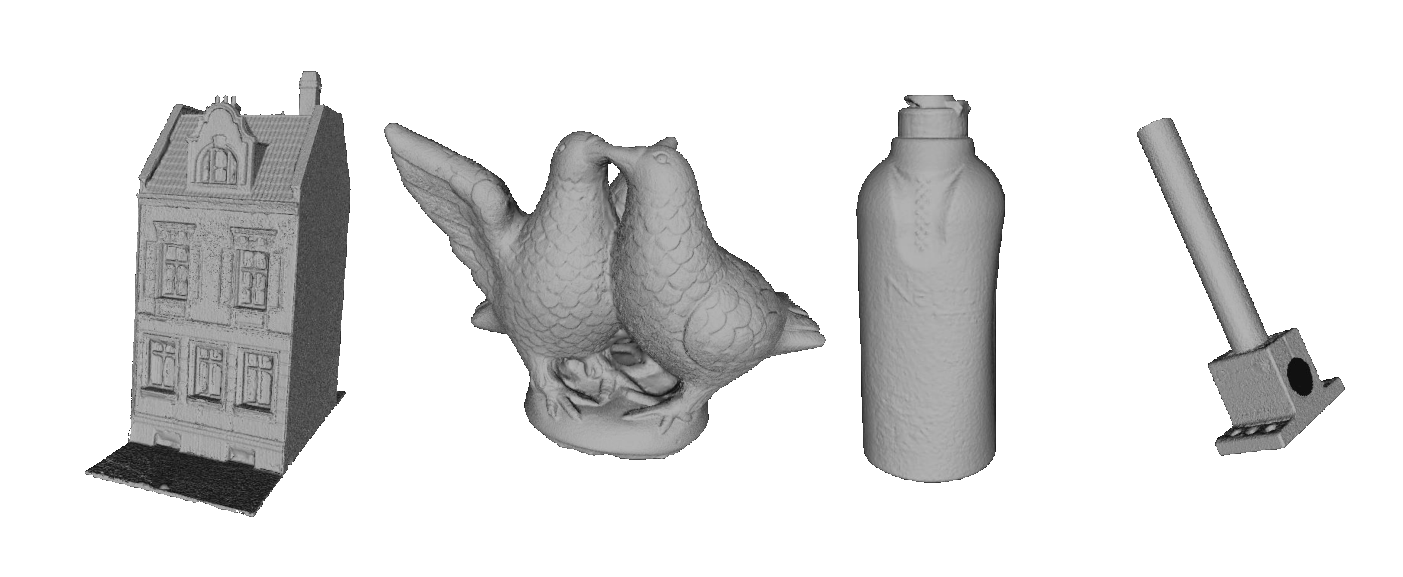
\includegraphics[clip, trim=1cm 1cm 1cm 1.3cm,width=0.9\linewidth, height= 0.4\linewidth, keepaspectratio]{img/objects/objects.pdf}
\caption{A sample of the scanned object models}
\label{fig:objects}
\end{figure}
All individual scan views are reconstructed by the Line shifting algorithm \cite{Guehring2000} which results in accurate and dense point cloud of the objects. Eleven temporal binary gray code patterns are projected followed by eight line shifting patterns. The point resolution of the scanned objects are in average 275 microns and consist of around 908000 vertices and 1.8 million faces in average. Once a single view of the model is scanned, noisy outliers of the measurement are manual removed and surface normals are estimated to ensure consistent normals. All 18 views are registered with Iterative Closest Point (ICP) and a new object frame is computed with principal component analysis on the point set. All models are sampled with a Poisson disk sampling algorithm \cite{Corsini2012} and triangulated with the poisson reconstruction algorithm \cite{Kazhdan2006} with an octree depth=14, solver divide = 8 and iso divide = 5. We use the PCL implementation \cite{RusuCousins2011}. All models are provided as coloured point clouds and triangular meshes, all in the $.ply$ format, see Figure \ref{fig:objects}. Note that the modelling setup is not radiometrical calibrated.

%Describe setup for scene aqusition
\subsection{Scene scanning}\label{sec:scene_scanning}
For the data collection we use a 6-axis ABB IRB 1600 industrial robot to provide a precise and highly repeatable camera pose. The robot is equipped with two PointGray Grasshopper3 GS3-U391S6C-C USB3 color cameras with resolution of 9.1 Mp and a Wintech Pro4500 projector with a resolution of 1140x912 pixels. The sensor cluster with the structured light sensor (SL) is mounted in the robot tool. 
%The sensor modalities are selected by two reasons. First, the structured light system (SL) ensure a high precision that is XX times better than the Kinect thus we are able to provide accurate ground truth pose data for each object in the scene down to a precision of xx mm. Second, Time-of-Flight sensors like the Kinect One sensor are popular sensors in many research areas such as robotic manipulation, 3D semantic mapping, people detection and consumer products thus we wanted to support the future development of 3D object recognition systems and algorithms by including the sensor in the dataset. 
%\begin{figure}[ht]
%\centering
%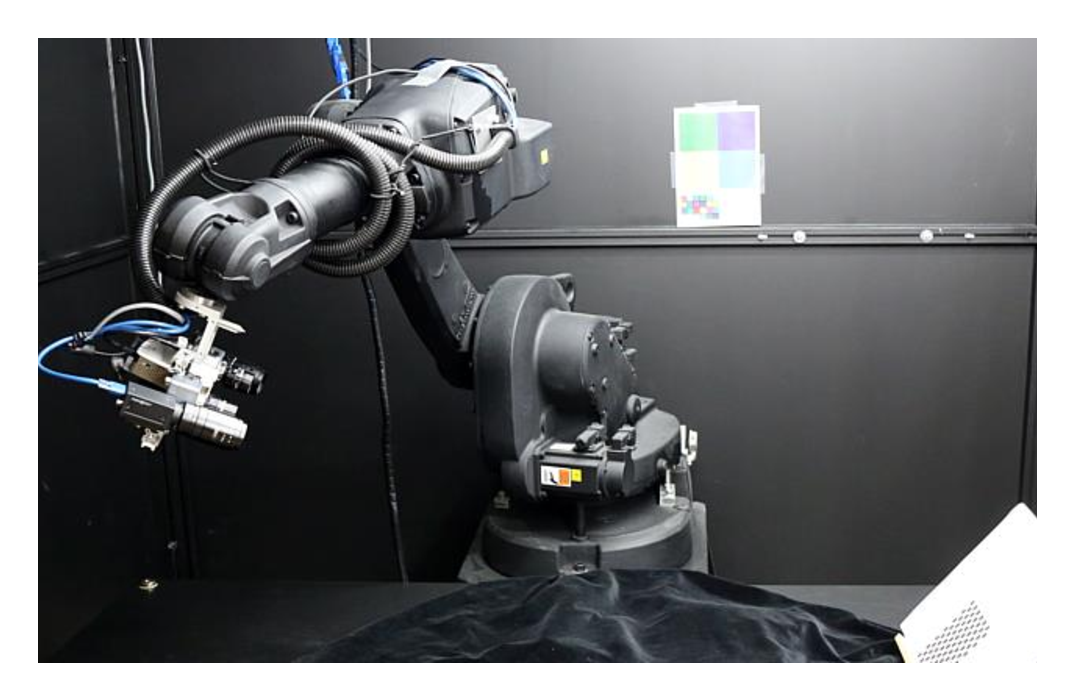
\includegraphics[width=0.9\linewidth, height= 0.6\linewidth]{Robot.pdf}
%\caption{Scan of the full scene with view frames}
%\label{fig:robot}
%\end{figure}
The Robot setup is constructed as a radiometric "dead" which gives a scene representation with zero ambient light. All scene illumination is controlled in the recording process. The sensor cluster is calibrated with an automatic calibration procedure which includes a stereo calibration of the SL sensor using \verb|OpenCV|\footnote{\url{http://opencv.org/}}.% and a intrinsic calibration of the Kinect using the \verb|iai_kinect2|\footnote{\url{https://github.com/code-iai/iai_kinect2}} software package. The Kinect calibration ensure a proper registration of the RGB values at each 3D point. 
An automatic hand eye calibration \cite{DornaikaHoraud1998} is conducted in order to align the structured light scans in the world frame. The world frame is placed in the robot base frame. Each physical scene is scanned from 11 different views with the structured line scanner (SL). During the structured light scanning process the chamber is completely dark in order to increase the signal-to-noise ration of the scan. The structured light scans are reconstructed with the Line shifting algorithm \cite{Guehring2000} with ten temporal pattern levels. The views are distributed equally on a quarter sphere around the scene, such that each scene is depicted from - 90 to 90 degrees horizontally and 0 to 45 degree vertically. The distance between the sensor views and the center of the scene is 0.8 meter. In order to be able to reproduce the results we store all images in raw Portable Network Graphics in full resolution (9.1 MP). De-bayering, white balance, image rectification, pattern decoding and point cloud reconstruction are a off line process.   
\begin{figure}[ht]
\centering
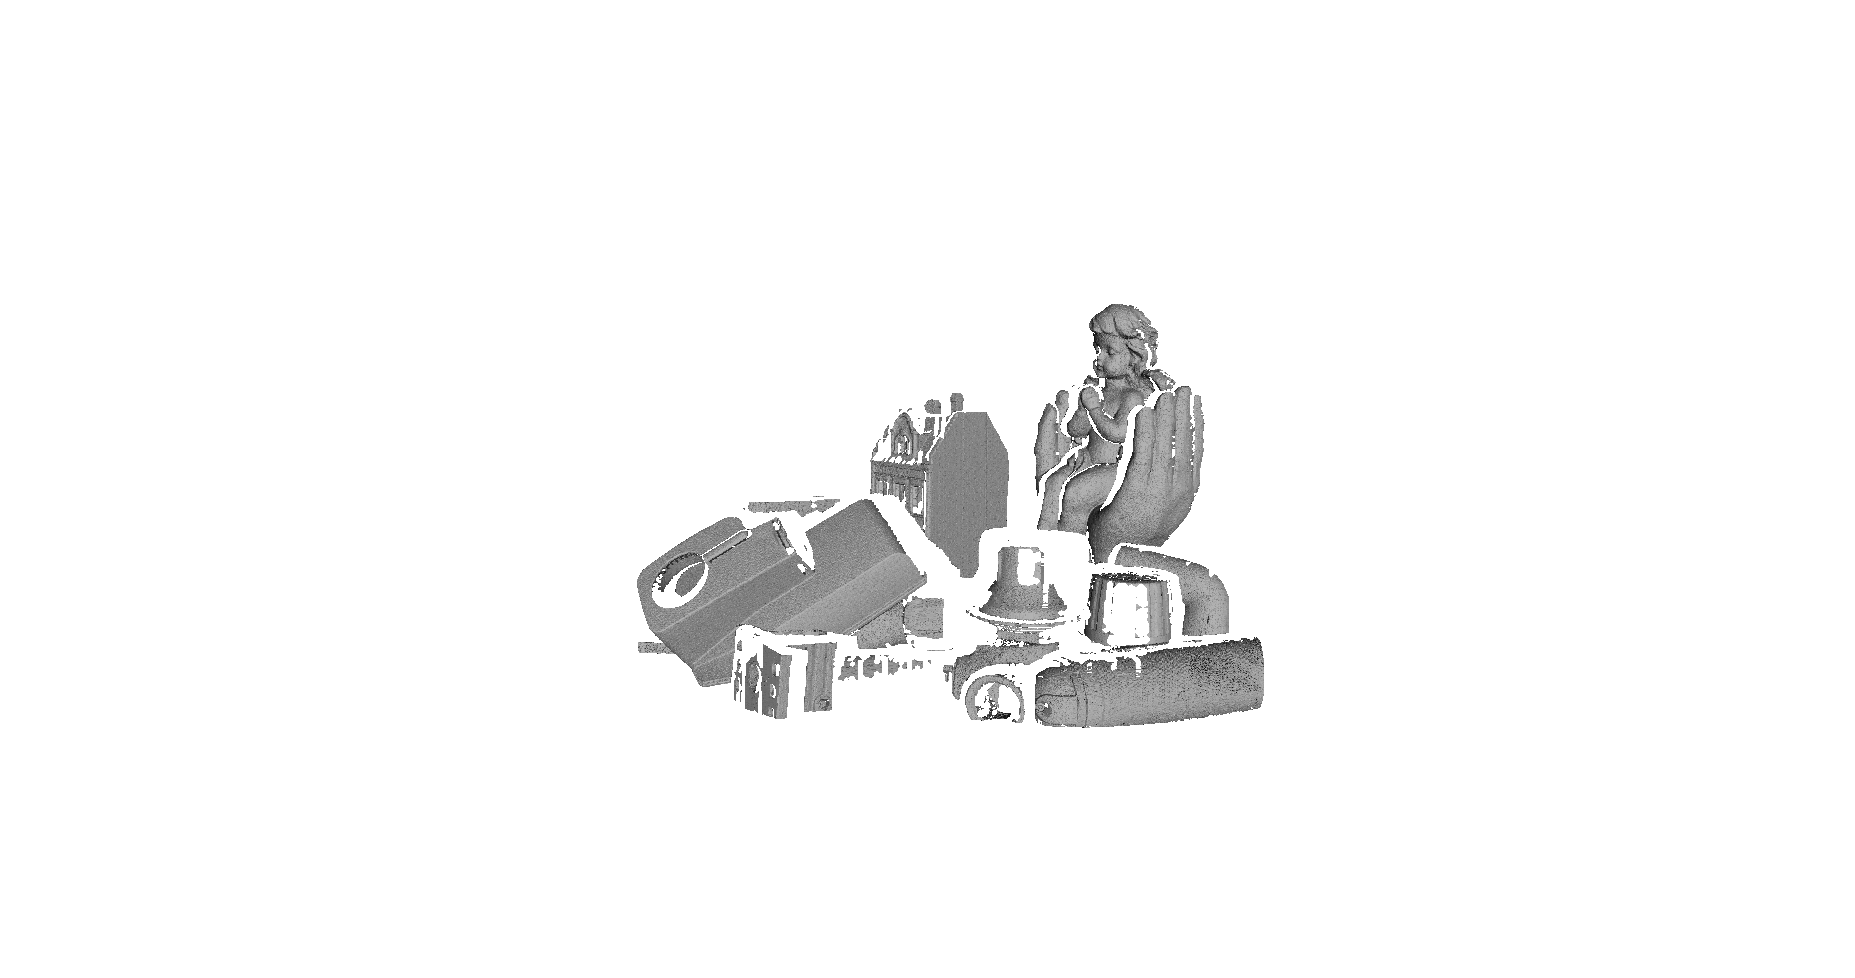
\includegraphics[clip, trim=14cm 6cm 13cm 8cm,width=1.0\linewidth, height= 1.0\linewidth, keepaspectratio]{img/mesh_scene.png}
\caption{Example on one of the 3200 triangulated scene}
\label{fig:mesh_scene}
\end{figure}
%Meshing of the scenes + normal estimation
Local shape features like 3D Tensor \cite{Mian2006}, ROPS \cite{Guo2013} and FPFH \cite{Fpfh2009} apply the underlying mesh surface during feature computation. In order for the dataset to support these algorithms all scenes are triangulated to a polygonal mesh. For each scene a set of corresponding triangles are computed with a 2D delaynay triangulation algorithm in VTK\footnote{\url{http://www.vtk.org/}}. Each $(x,y)$ point coordinates of the scene point cloud are normalized with its $z$ component in order to project the 3D point cloud into 2D and triangulated. The 3D mesh structures are created by re-assigning all 3D point with the triangles of the same index. Long edges in the mesh are then removed form the mesh in order to avoid triangles between step edges. An example of a triangulated scene is shown in Figure \ref{fig:mesh_scene}.
%A Note on ground truth
\subsection{Ground Truth 6D pose}\label{sec:gt_pose}
For each of the 3200 scenes the 6D ground truth pose, occlusion and clutter estimates for each object are provided. We estimate the occlusion from Equation \ref{eq:occlusion} and clutter from Equation \ref{eq:clutter} by counting the number of points at the object model in which the squared euclidean distance to a scene point is less than two times the scene resolution. Both the object model and the scene are sampled to ensure equal point distance.
\begin{equation}
Occlusion = 1 - \frac{visible \: object \: points }{total \: object \: points} 
\label{eq:occlusion}
\end{equation}
\begin{equation}
Clutter = 1 - \frac{visible \: object \: points}{total \: scene \: points}
\label{eq:clutter}
\end{equation}
\indent
Accurate ground true poses are ensured by manual annotation of each object in the scenes. First, one point cloud that covers 180 degree of the scene is stitched together form each of the 11 views and registered with ICP. This full scene point cloud is applied in the annotation process, see Figure \ref{fig:scene}. The full scene point cloud covers the geometric structures of each model in the scene with more point compared to the individual views. Thus, it is possible to get a more accurate ICP registration of the object model in the scenes. All 290 combined scenes are manual annotated by selecting four identical points for each model and the scene, followed by an estimation of the rigid transform. An iterative ICP, which incremental decreases the allowed correspondence distance ensures a very accurate final ground truth pose of each object in the scene. The final ICP iterations are accomplished with the full resolution model to get the best fit of the model points to the scene points. The individual ground truth poses in each sensor view $T_{sensor_{n}}$ is computed by transforming the ground truth poses from the world frame $T_{world}$ to each of the individual sensor frames $T_{sensor_{n}}$. Equation \ref{eq:transformation} show the final transformation. 
\begin{equation}
T^{world}_{sensor_{n}} = T^{-1}_{robot} \cdot T^{-1}_{HandEye} \cdot T^{-1}_{icp} \cdot T_{gt}
\label{eq:transformation}
\end{equation}
where $T_{robot}$ is the known robot pose for each view point, $T_{HandEye}$ is the calibrated hand eye transform, $T_{icp}$ is the alignment transform which align view $n$ to view $0$ in the world frame and $T_{gt}$ is the annotated ground truth pose in the full scene point cloud with the world frame as reference. This methodology guarantees accurate pose in $T{sensor_{n}}$ independent of the amount of occlusion. Even in views with limited number of scene points of an object the ground truth pose is accurate because the ground truth pose is computed in the full scene point cloud. For each ground truth pose in each sensor view, we compute the RMS error between the model and the scene to guarantee the overall accuracy of all ground truth poses. On average the RMS error of all ground truth poses is within 0.15 mm.   
%-------------------------------------------------------------------------
\section{Benchmark}\label{sec:benchmark}
This section outlines the experimental protocol defined to validate the dataset. The protocol is inspired by Salti \etal \cite{Salti2014}. The evaluation is divide into two parts; feature matching accuracy and object recognition rate. The selected local feature descriptors for our evaluation include; Spin Image (SI) \cite{Johnson1999}, PFH \cite{Rusu2008}, FPFH \cite{Fpfh2009}, USC \cite{usc2010}, SHOT \cite{Tombari2010}, ROPS \cite{Guo2013}, ECSAD \cite{Ecsad2015} and NDHIST \cite{Buch2016}. The features are selected based on implementation availability and results from previous studies on feature descriptor benchmarking \cite{Guo2015},\cite{Buch2016}. 
\subsection{Feature Matching}\label{sec:benchmark_matching}
The descriptiveness and accuracy of a feature descriptor are measured with Precision-Recall and presented as 1-Precision vs. Recall Cruves (PRC). First we sample both the query models and the target scenes with a voxel grid sampling \cite{RusuCousins2011} which results in equal point distance. The voxel size is tuned to give approximately 1000 seed points per. object in both the query and target. The target seed points are found by transforming the query seeds into the target by applying the object ground truth pose. The target seeds are selected in a nearest neighbour search with a distance threshold. A feature descriptor for each seed point in the query and target mesh is computed.  For fair comparison individually tuned support radii for each descriptors are used. We use the following feature resolution multiplier: SI($20$), 3DSC($22.5$), FPFH($17.5$), USC($25$), SHOT($17.5$), ROPS($20$), ECSAD($20$), NDHIST($31$). Hence, the radius for each feature is a function of the average model or scene resolution. Upon feature computation the underlying scene and object meshes are utilized in 0.25 and 0.05 decimated version; respectively. The level of decimation are empirical determined to the level with best overall matching results for all features. During decimation the normal orientation is re-computed for each vertex by the area weighted mean of the mesh triangle \cite{Thurmer1998} and normalized. In order to resolve the exact number of correct feature matches, a brute-force linear kd-tree search is	 used with a ${L_2}$ distance function. Other distance metrics such as ${L_1}$, ${L_\infty}$, are tested in previous work but the best results are achieved with the $L_2$ distance metric. Thus, we only present results for the ${L_2}$ metric. During matching we are computing the ratio of the nearest and the second-nearest matching distances. This matching strategy is adapted from multiple previous studies e.g. Lowe \etal \cite{Lowe2004} that proved a performance enhancement compared to a native matching strategy where only the nearest neighbour is considered. 
Once all matches for all queries are computed they are ranked and sorted according to the ${L_2}$ distance in one array. The correct matches are found by traversing the array of matches and count the number of matches that are spatial close, determined by a distance threshold. The PRC curves are presented in Section \ref{sec:evaluation} where precision refers to the number of correct matches compared to the total number of matches. Recall refers to the number of correct matches compared to the total amount of possible matches (i.e. feature seed points found in the target). In addition to PRC curves, we compute the area under the PRC curve (AUC) as a single quantitative measure of the overall accuracy. The AUC is computed as the numerical integration over all (P,R) per feature. %and the formula is presented in Equation \ref{eq::maxf1}.
%Ratio of the nearest matching feature distance to that of the second nearest \cite{Buch2016}  
%\begin{equation}\label{eq::maxf1}
%max F_1 = {max}_{(P,R)} \left(2 \cdot \frac{P\cdot R}{P+R}\right)
%\end{equation}
\subsection{Pose estimation}\label{sec:pose_estimation}
In this section the experimental protocol for the pose estimation experiments is presented. The sampling and seed point selection are identical with the feature matching benchmark presented, except that we cannot use the ground truth pose for selecting target seed points. Instead, the target resolution is doubled, to quadruples the number of feature descriptors which increase the chance for describing the same feature. To increase the efficiency during matching we apply approximate nearest neighbour search to determine correspondences hypotheses instead of exact matching. Again, the ratio of the nearest and second nearest neighbours feature distances are used. A multiple randomized kd-trees with a bound of 512 checks and 4 trees are used as a good trade-off between accuracy and efficiency. Correspondences are ranked by the ${L_2}$ distance which inputs potential feature correspondences to a hypothesis and test RANSAC algorithm.
During random sampling, three correspondences are sampled which is sufficient to generate a hypothesis pose. The hypothesis pose is tested by transforming the query points and counting the number of query points close to the target feature up to a tolerance given by the inlier threshold. The algorithm filters out false positives by setting a lower minimum of the number of inliers required to accept a pose hypothesis to 1\%. The pose with the highest number of inliers is returned as the object pose. Our RANSAC implementation deviates from classic RANSAC, which treats all data points uniformly. Instead we sample correspondences according to their quality score. The quality scores are given by the negative normalized ${L_2}$ distance ratio. The efficiency of the algorithm is further increased by only considering the top 10\% of the best correspondences with the highest quality score before running the RANSAC algorithm. Upon RANSAC completion the final pose is refined by 150 ICP iterations on the query/target seed points. We accept a pose estimate as valid by computing the euclidean and geodesic distances between the computed pose and the ground true pose from the annotation process. If the euclidean and geodesic distances are less than the threshold the object is correctly recognized. The euclidean and geodesic distance metrics are computed in accordance to Equation \ref{eq::rot} and \ref{eq::trans}.      
\begin{equation}\label{eq::rot}
arccos \left(\frac{trace(\textbf{R}^{T}\hat{\textbf{R}})-1}{2}\right) \leq 7.5^\circ
\end{equation}
\begin{equation}\label{eq::trans}
||\textbf{t} - \hat{\textbf{t}} || \leq 5mm
\end{equation}
The recognition rate is computed as the ratio of true positive poses compared to all detected poses as a quantitative measure of the overall recognition performance.
%-------------------------------------------------------------------------
\section{Evaluation}\label{sec:evaluation}
In this section we present the results of our evaluation benchmark. All experiments are based on the proposed dataset where 3204 scenes, 45 objects and 5675 ground truth poses are included. As a first evaluation we benchmark the matching accuracy of the seven feature descriptors with the parameters outlined in Section \ref{sec:benchmark_matching} and all 45 object models included. The PRC curve of the overall matching accuracy is presented in Figure \ref{fig:all_L2_RATIO_zoom}.   
\begin{figure}[h]
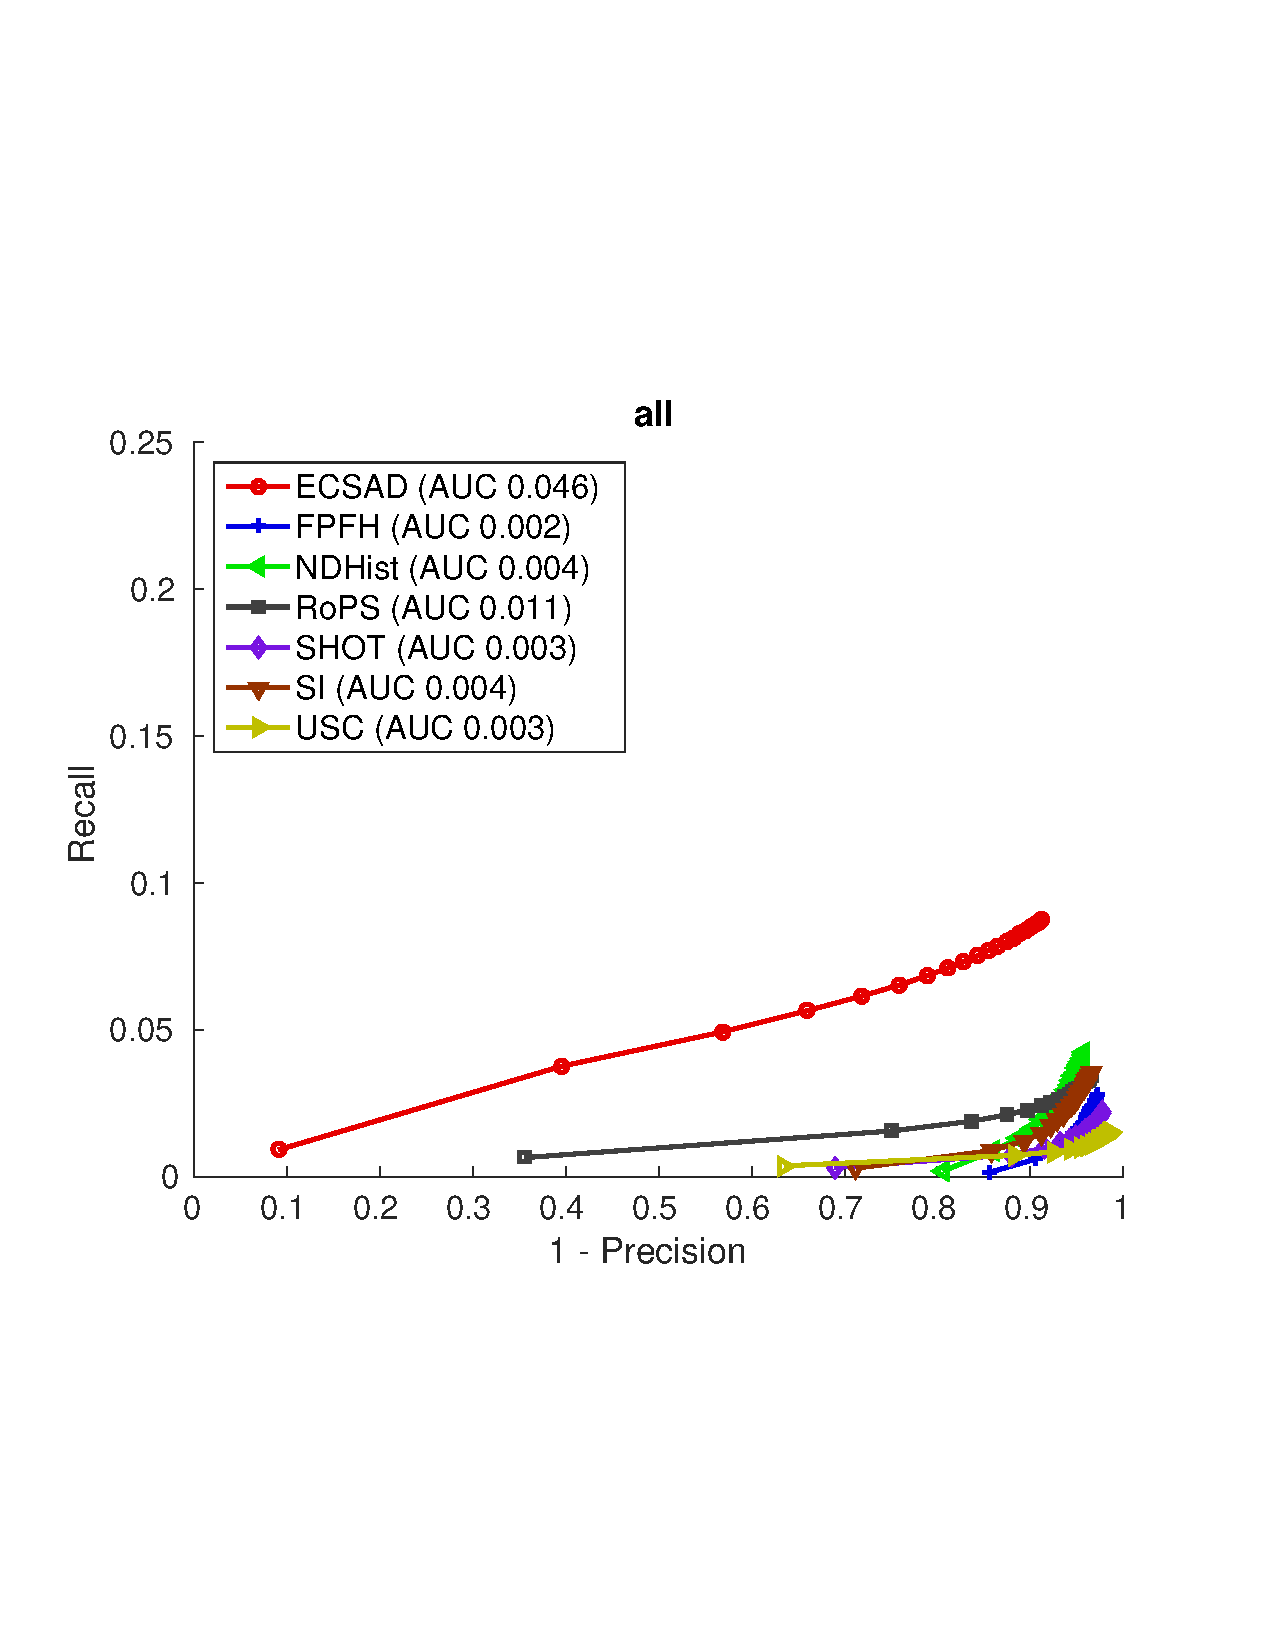
\includegraphics[clip, trim=0.7cm 6cm 0.7cm 6cm,width=1.0\linewidth, height= 1.0\linewidth, keepaspectratio]{img/all_L2_RATIO_zoom.pdf} 
\caption{Overall PRC curve}\label{fig:all_L2_RATIO_zoom}
\end{figure}
As expected the total matching accuracy is much lower compared to previous studies e.g. Guo \etal \cite{Guo2015} and Buch \etal \cite{Buch2016}, which both are running a similar benchmark but on previous proposed datasets. The result indicate that our objective of the proposed dataset has been fulfilled. Moreover, the evaluation shows that the ECSAD feature has a best performance with a AUC = 0.046 followed by ROPS with AUC = 0.011. In order to investigate the performance further we run the matching benchmark for each object model and compute PRC curves for each of the 45 models. We have categorize the object into three different groups and present 3 PRC curves for each group in Figure \ref{fig:angel}-\ref{fig:noise} as a sample. The three groups are a) Geometric complex objects, b) Cylindrical objects and c) Flat or box shaped objects. The objects that corresponds to the PRC curves in Figure \ref{fig:angel}-\ref{fig:noise} are presented in Figure \ref{fig:selected_objects}. The geometric complex objects are the Angel, the Birds and the Rabbit in Figure \ref{fig:selected_objects}(a)-(c), the cylindrical objects are Neutral, Pringles and Hand soap in Figure \ref{fig:selected_objects}(d)-(f), and the flat or box shaped objects are the button, the brake disc and the Psu in Figure \ref{fig:selected_objects}(g)-(i). The results show that a recent precision and recall are achieved with the Angel,Birds and Rabbit, but it is much lower than previous studies e.g. Buch \etal \cite{Buch2016} that obtain very matching accuracy for some datasets. These low numbers for our geometric ideal objects indicate that the proposed dataset have the desired level of complexity.     Regarding, the cylindrical objects which features the Neutral, Pringles and Hand Soap objects, it is clear that current local shape descriptors is very little descriptive for these uniform shaped objects. Again, ECSAD performs in general best which might results from the fact that ECSAD describes edges in a good way. For the flat and boxed shaped models we can conclude that current state of the art feature descriptors is not suitable as the only detection method.\\ 	
\indent The result for the pose estimation experiments are presented in Table \ref{tab:recognition} and Figure \ref{fig:pose_est_results}. Our object recognition pipeline in these experiment is in accordance to the presented pipeline in Section \ref{sec:pose_estimation}. 
\newcolumntype{P}[1]{>{\centering\arraybackslash}p{#1}}
\begin{table*}[t]
\centering
\scalebox{0.8}{
\begin{tabular}{p{1.25cm} | P{1.1cm} | P{1.4cm} P{1.4cm} P{1.4cm} P{1.4cm} P{1.4cm} P{1.7cm} P{1.4cm} P{1.65cm} P{1.4cm} | P{1.4cm}}
\hline
\textbf{Feature} & \textbf{Overall} & \textbf{Angel} & \textbf{Birds} & \textbf{Rabbit} & \textbf{Neutral} & \textbf{Pringels} & \textbf{Hand soap} & \textbf{Button} & \textbf{Brake Disc} & \textbf{Psu}  & \textbf{\textit{Mean ($\lambda$)}} \\
\hline
\hline
 \textbf{\textit{ECSAD}}  & 0.21  & \textbf{0.59} & \textbf{0.86} & \textbf{0.62} & 0.00 & 0.06 & 0.03 & 0.00 & 0.00 & 0.00 & 0.00\\
 \textbf{\textit{FPFH}}   & 0.01  & 0.07 & 0.01 & 0.04 & 0.00 & 0.00 & 0.02 & 0.00 & 0.00 & 0.00 & 0.00\\
 \textbf{\textit{NDHIST}} & 0.02  & 0.13 & 0.05 & 0.14 & \textbf{0.02} & \textbf{0.06} & 0.02 & 0.00 & 0.00 & 0.00 & 0.00\\
 \textbf{\textit{ROPS}}   & 0.13  & 0.45 & 0.70 & 0.29 & 0.01 & 0.00 & 0.00 & 0.00 & 0.00 & 0.00 & 0.00\\
 \textbf{\textit{SHOT}}   & 0.04  & 0.25 & 0.09 & 0.14 & 0.00 & 0.00 & 0.00 & 0.00 & 0.00 & 0.00 & 0.00\\
 \textbf{\textit{SI}}     & 0.05  & 0.20 & 0.16 & 0.10 & 0.01 & 0.00 & 0.00 & 0.00 & 0.00 & 0.00 & 0.00\\
 \textbf{\textit{USC}}    & 0.00  & 0.01 & 0.04 & 0.09 & 0.00 & 0.00 & 0.00 & 0.00 & 0.00 & 0.00 & 0.00\\
%\textbf{\textit{PFH}}    & 0.00 \vline  & 0.00 & 0.00 & 0.00 & 0.00 & 0.00 & 0.00 & 0.00 & 0.00 & 0.00\\
%\textbf{\textit{3DSC}}   & 0.00 \vline  & 0.00 & 0.00 & 0.00 & 0.00 & 0.00 & 0.00 & 0.00 & 0.00 & 0.00\\
 \hline
\end{tabular}
}
\caption{Overall recognition rates. \textbf{Column 1:} Features descriptors. \textbf{Column 2:} Overall recognition rate. \textbf{Column 3-11:} Recognition rate for each sample object in Figure \ref{fig:selected_objects}. \textbf{Column 12:} Mean recognition rate for the 9 sample object per. feature.}
\label{tab:recognition}
\end{table*}
\begin{figure*}[t]
	\centering
	\begin{subfigure}[Ecsad]{%{0.18\textwidth}
		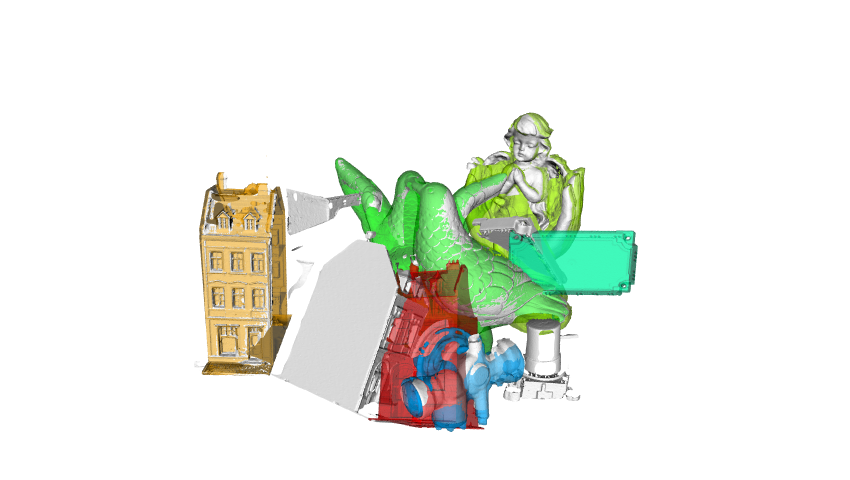
\includegraphics[clip, trim=6.7cm 1cm 6.7cm 3.5cm,width=0.3\linewidth, height= 0.2\linewidth, keepaspectratio]{img/ecsad_1.png}
		%\subcaption{Angel}\label{fig:stl_n3}
		}
	\end{subfigure}
	\begin{subfigure}[Ndhist]{%{.18\textwidth}	
		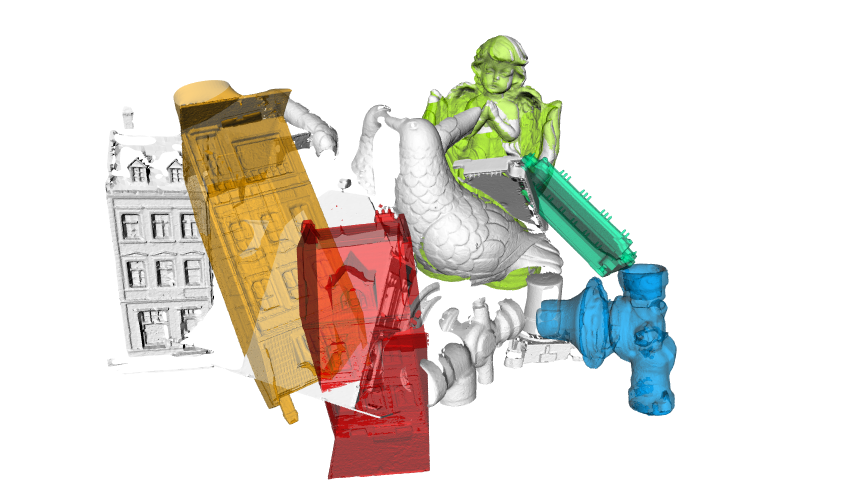
\includegraphics[clip, trim=5cm 1cm 5cm 1cm,width=0.3\linewidth, height= 0.2\linewidth, keepaspectratio]{img/ndhist.png}
		%\caption{Birds}\label{fig:stl_n3}
		}
	\end{subfigure}
	\begin{subfigure}[Rops]{%{.18\textwidth}
		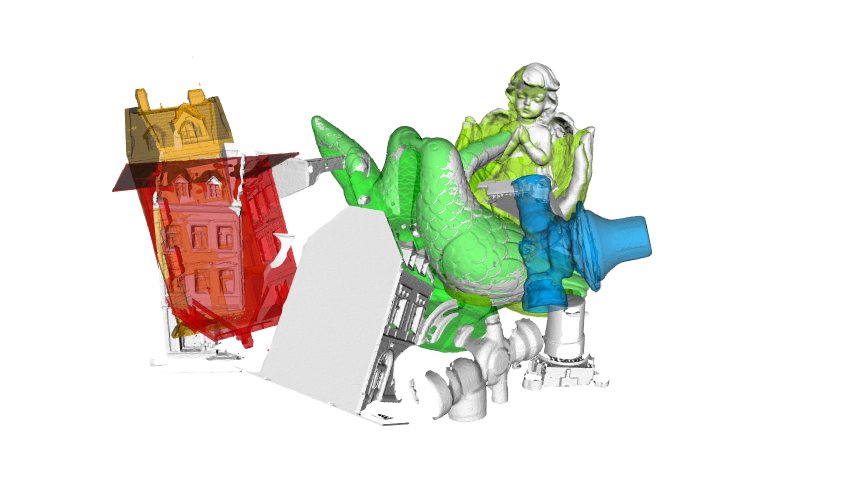
\includegraphics[clip, trim=4cm 1cm 7cm 1.7cm,width=0.3\linewidth, height= 0.2\linewidth, keepaspectratio]{img/rops.png}
		%\subcaption{Rabbit}\label{fig:stl_n3}
		}
	\end{subfigure}
	\\
	\begin{subfigure}[Shot]{%{.18\textwidth}	
		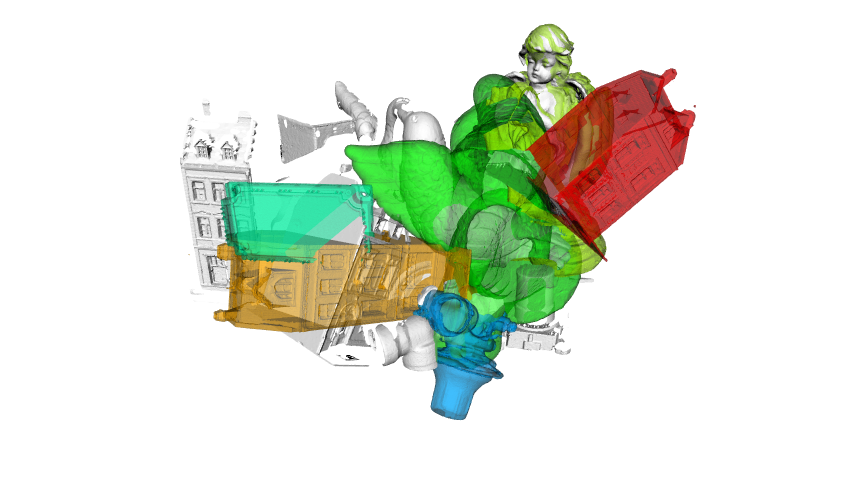
\includegraphics[clip, trim=6cm 2cm 5cm 0.8cm,width=0.3\linewidth, height= 0.2\linewidth, keepaspectratio]{img/shot.png}
		%\caption{Noise level 3 for STL dataset}\label{fig:stl_n3}
		}
	\end{subfigure}
	\begin{subfigure}[Fpfh]{%{.18\textwidth}
		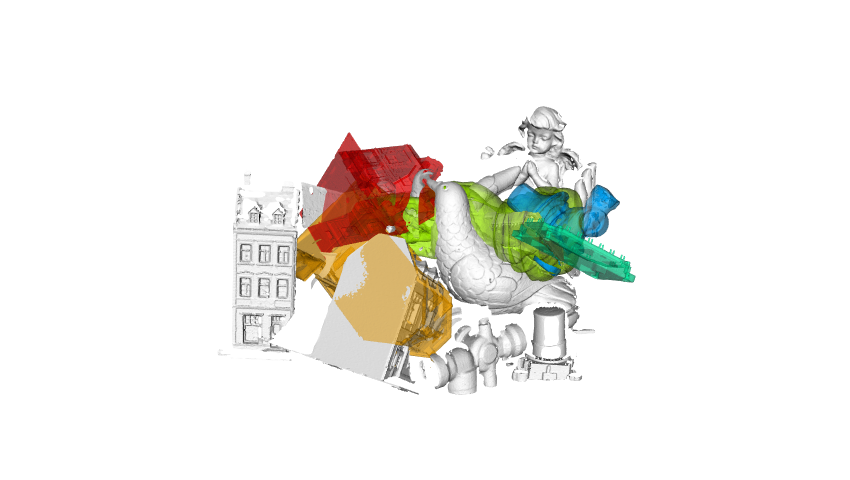
\includegraphics[clip, trim=7.2cm 2cm 7.2cm 3.3cm,width=0.3\linewidth, height= 0.2\linewidth, keepaspectratio]{img/fpfh.png}
		%\caption{Noise level 3 for STL dataset}\label{fig:stl_n3}
		}
	\end{subfigure}
	\begin{subfigure}[Spin images]{%{.18\textwidth}
		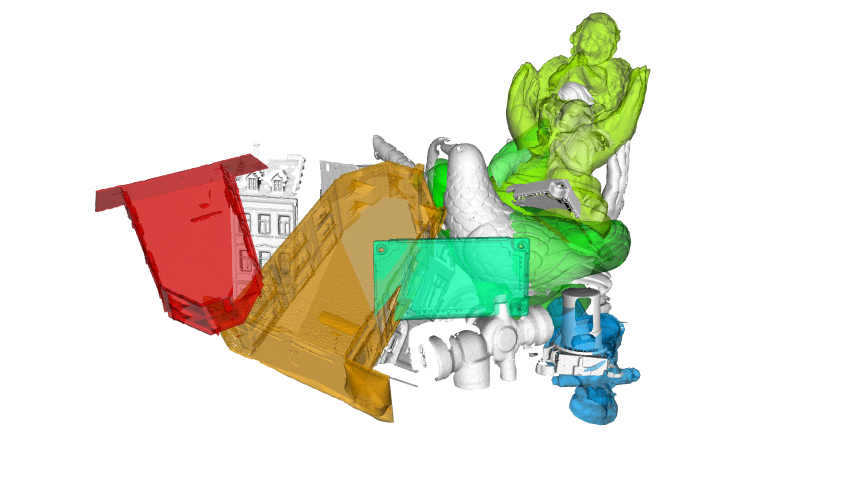
\includegraphics[clip, trim=4.2cm 2cm 6cm 0.2cm,width=0.3\linewidth, height= 0.2\linewidth, keepaspectratio]{img/si.png}
		%\caption{Noise level 3 for STL dataset}\label{fig:stl_n3}
		}
	\end{subfigure}
%	\begin{subfigure}[Usc]{%{.18\textwidth}
%		\fbox{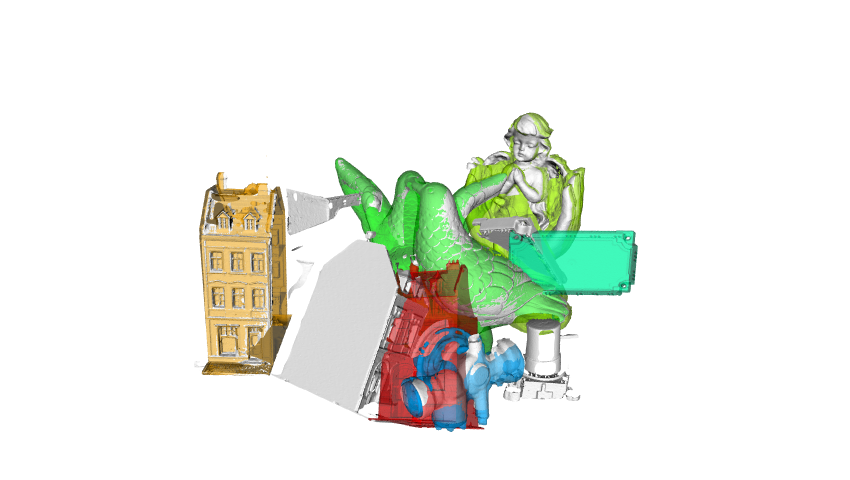
\includegraphics[clip, trim=6cm 1cm 5cm 1cm,width=0.2\linewidth, height= 0.25\linewidth, keepaspectratio]{img/ecsad_1.png}}
%		%\caption{Noise level 3 for STL dataset}\label{fig:stl_n3}
%		}
%	\end{subfigure}
	\captionsetup{justification=centering}
\caption{Qualitative recognition results for scene 8}\label{fig:pose_est_results}
\end{figure*}
In the first recognition experiment we run the pipeline with all 45 object model included and present the recognition rate in Table \ref{tab:recognition}, second column. In the second experiment we run the recognition benchmark for each individual object, which is a harder problem because we remove scene points upon each detected object. Hence, we reduce the number of scene point for each match even when the algorithm recognize false positives which results in removal of false point in the scene. Again, as expected Ecsad and Rops performs best on average. However, the recognition rate is lower than seen in other datasets which is expected since some views in our dataset is heavy occluded. In Figure \ref{fig:pose_est_results} qualitative results are presented for the recognition result in scene 8. Again, is is clear that Ecad and rops performing best with 4 and 2 correct recognize object, respectively.      

\section{Discussion \& Conclusion}\label{sec:conclusion}
This paper has introduce a new large scale dataset for 3D object recognition and a evaluation benchmark to validate the dataset. Our benchmark results show as expected low matching scores for repetitive and symmetric objects. Further, objects with non-distinctive local geometric areas and thin edges results as expected in very low matching quality. From the evaluation we conclude that the dataset full-fill our requirement in terms of difficulty and that the objects ans scenes included represent the real world problems that a 3D object recognition system will face in the future. Our main goal of this work has been to span the real world 3D object recognition challenge that we face in especially in the flexible robotic automation industry.\\



\clearpage
\begin{figure*}[htp]
	\centering
	\begin{subfigure}[Angel]{%{0.18\textwidth}
		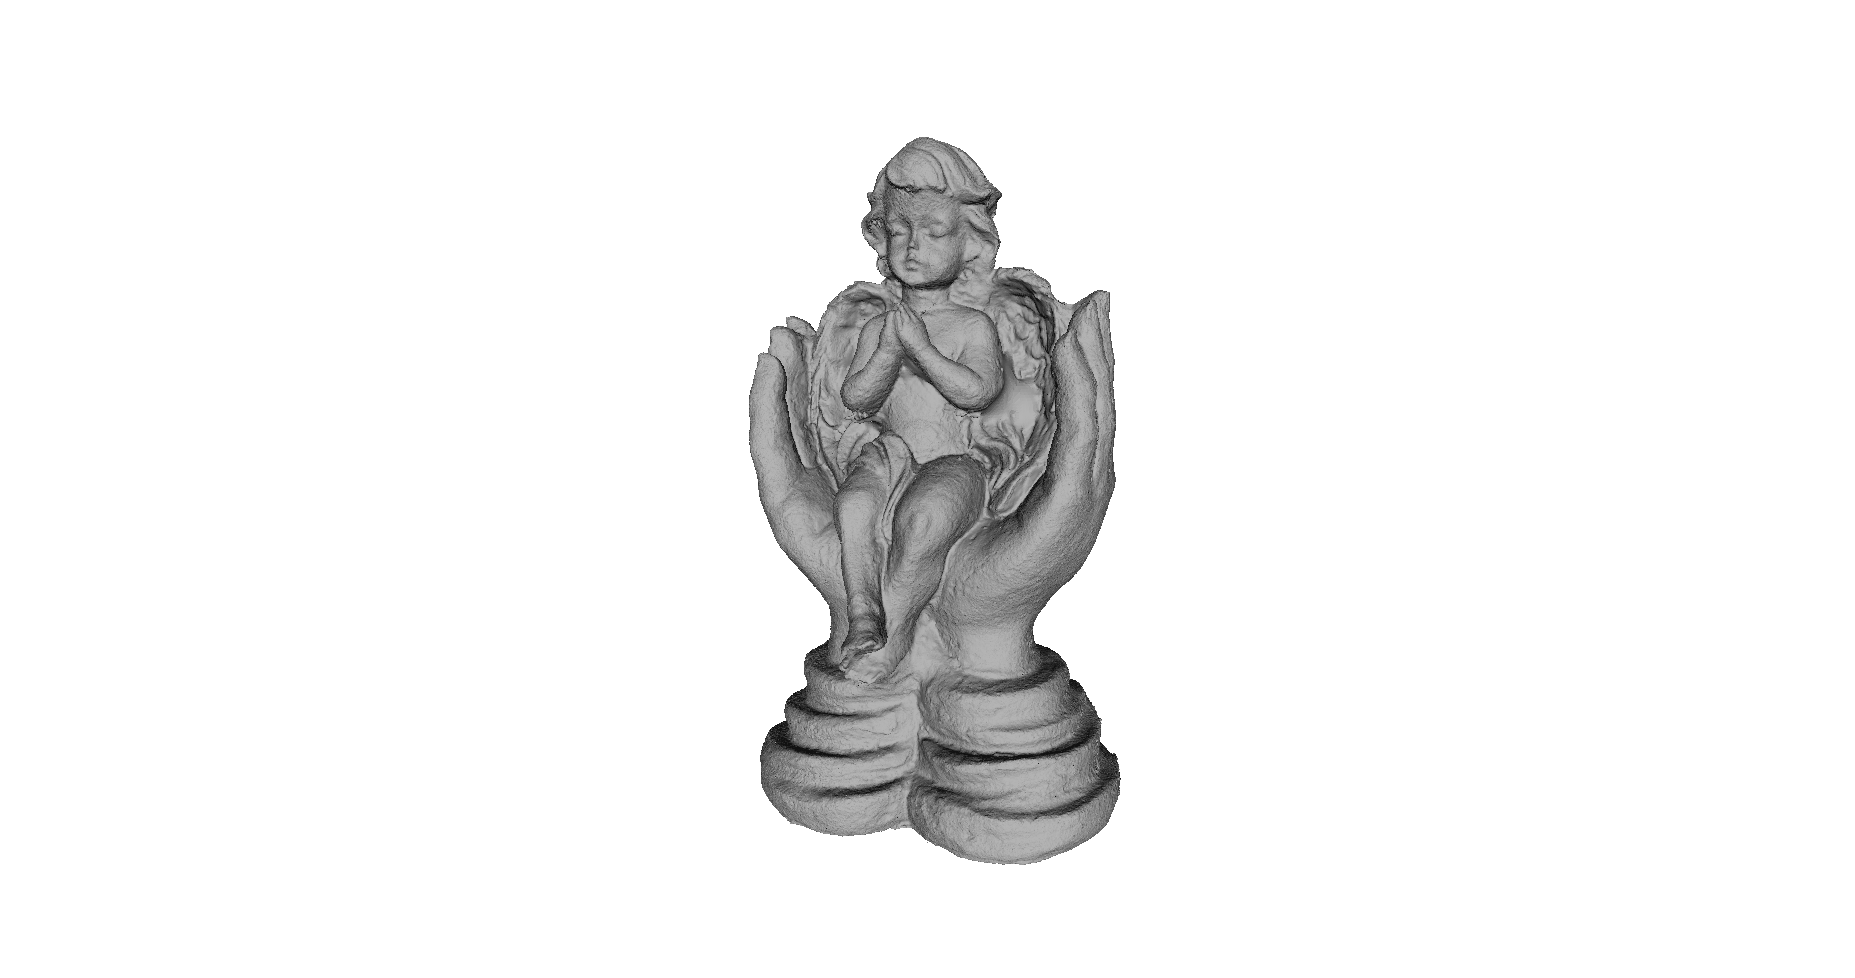
\includegraphics[clip, trim=12cm 2cm 12cm 2cm,width=0.12\linewidth, height= 0.12\linewidth, keepaspectratio]{img/snapshot04.png}
		%\subcaption{Angel}\label{fig:stl_n3}
		}
	\end{subfigure}
	\begin{subfigure}[Birds]{%{.18\textwidth}	
		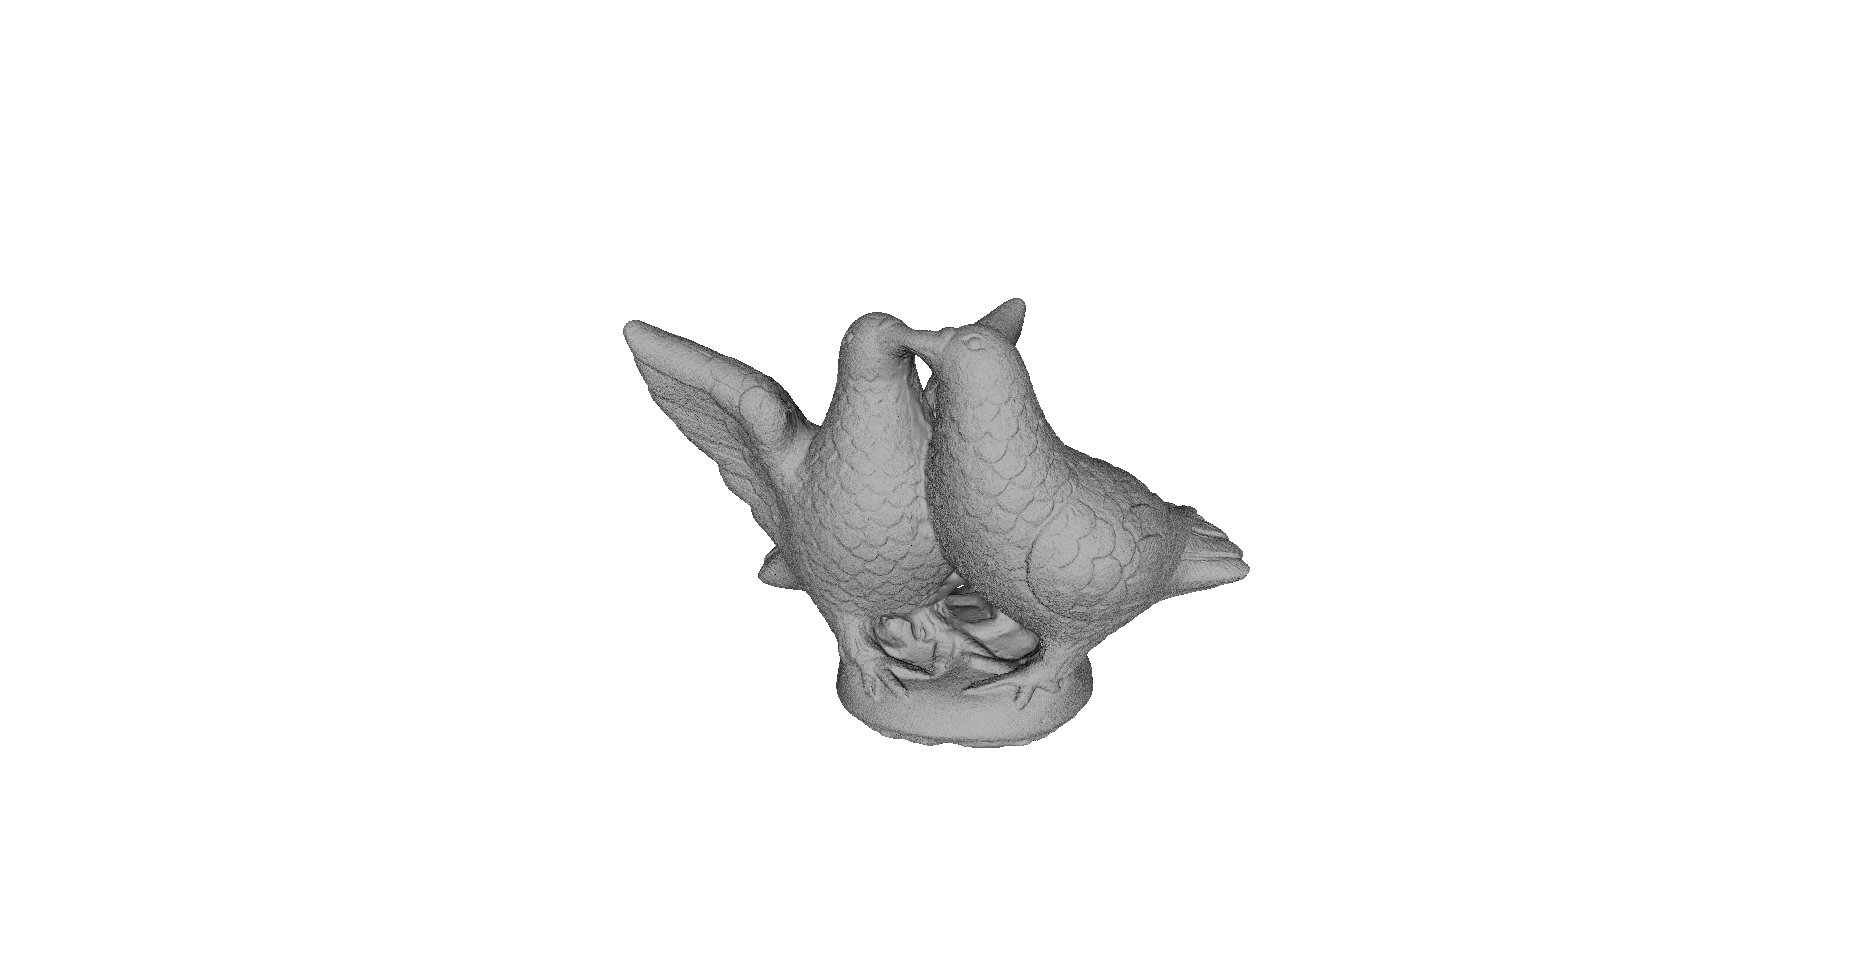
\includegraphics[clip, trim=12cm 2cm 12cm 2cm,width=0.12\linewidth, height= 0.12\linewidth, keepaspectratio]{img/snapshot05.png}
		%\caption{Birds}\label{fig:stl_n3}
		}
	\end{subfigure}
	\begin{subfigure}[Rabbit]{%{.18\textwidth}
		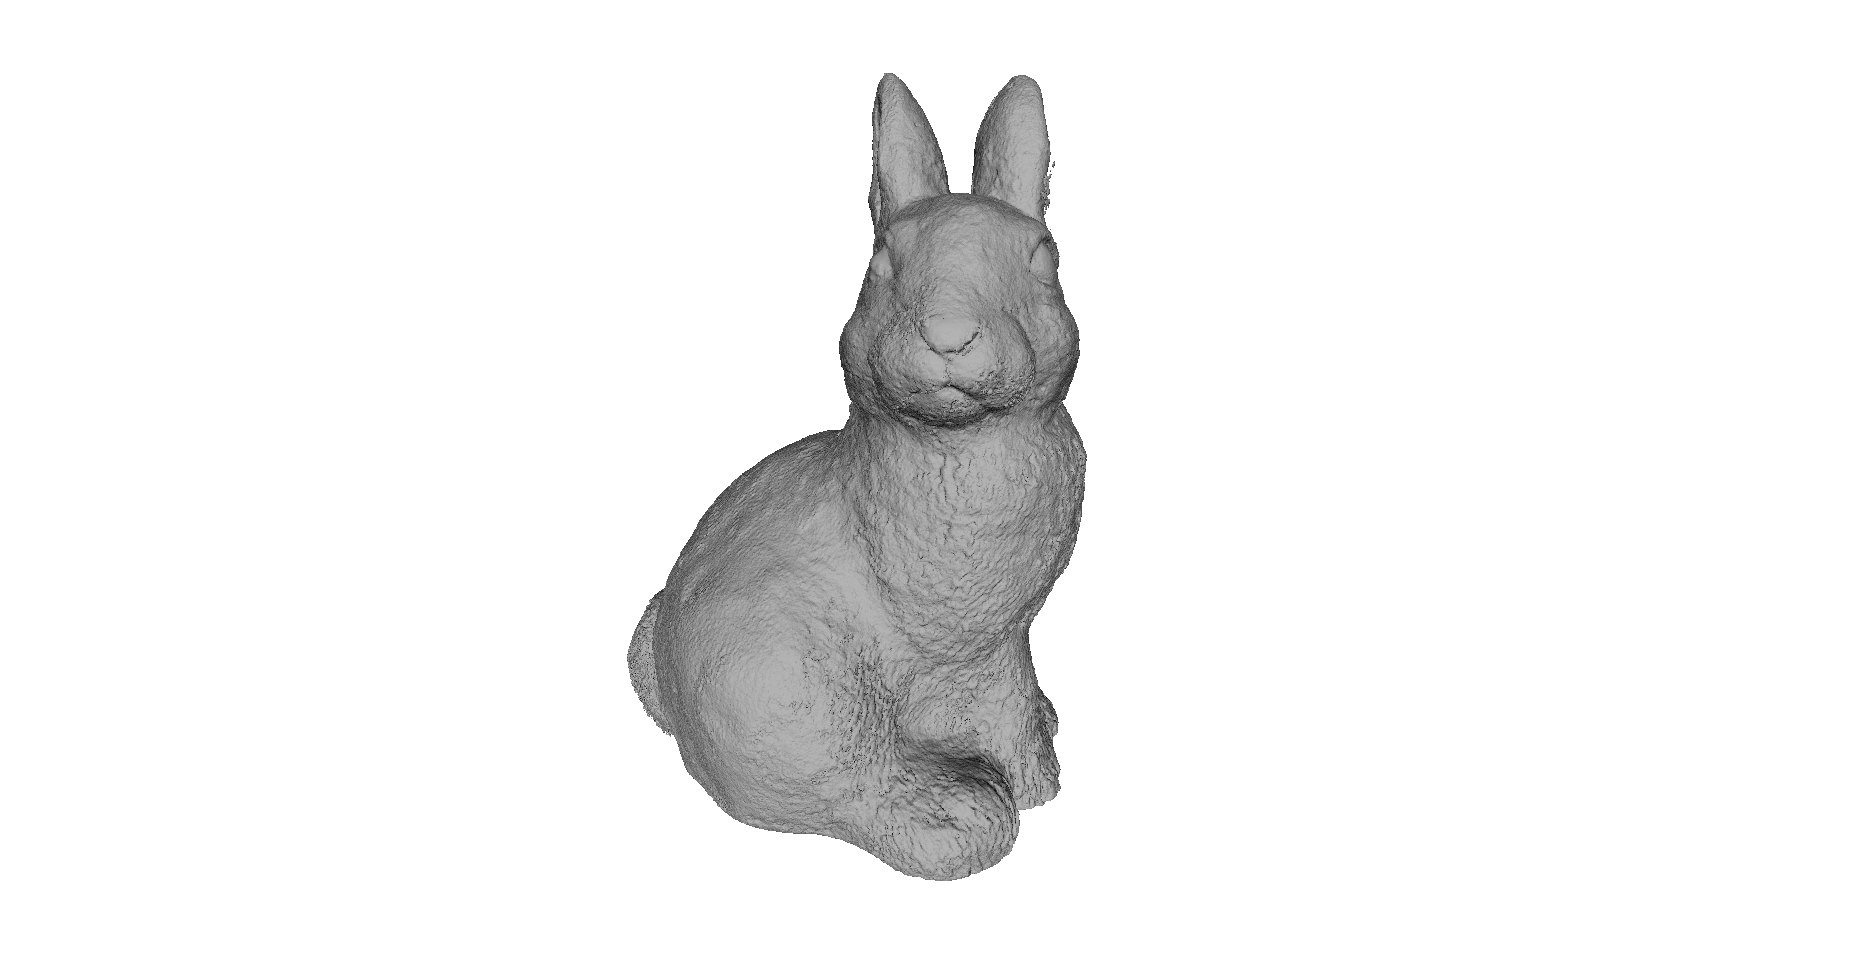
\includegraphics[clip, trim=12cm 2cm 12cm 2cm,width=0.12\linewidth, height= 0.12\linewidth, keepaspectratio]{img/snapshot07.png}
		%\subcaption{Rabbit}\label{fig:stl_n3}
		}
	\end{subfigure}
	\begin{subfigure}[Neutral]{%{.18\textwidth}	
		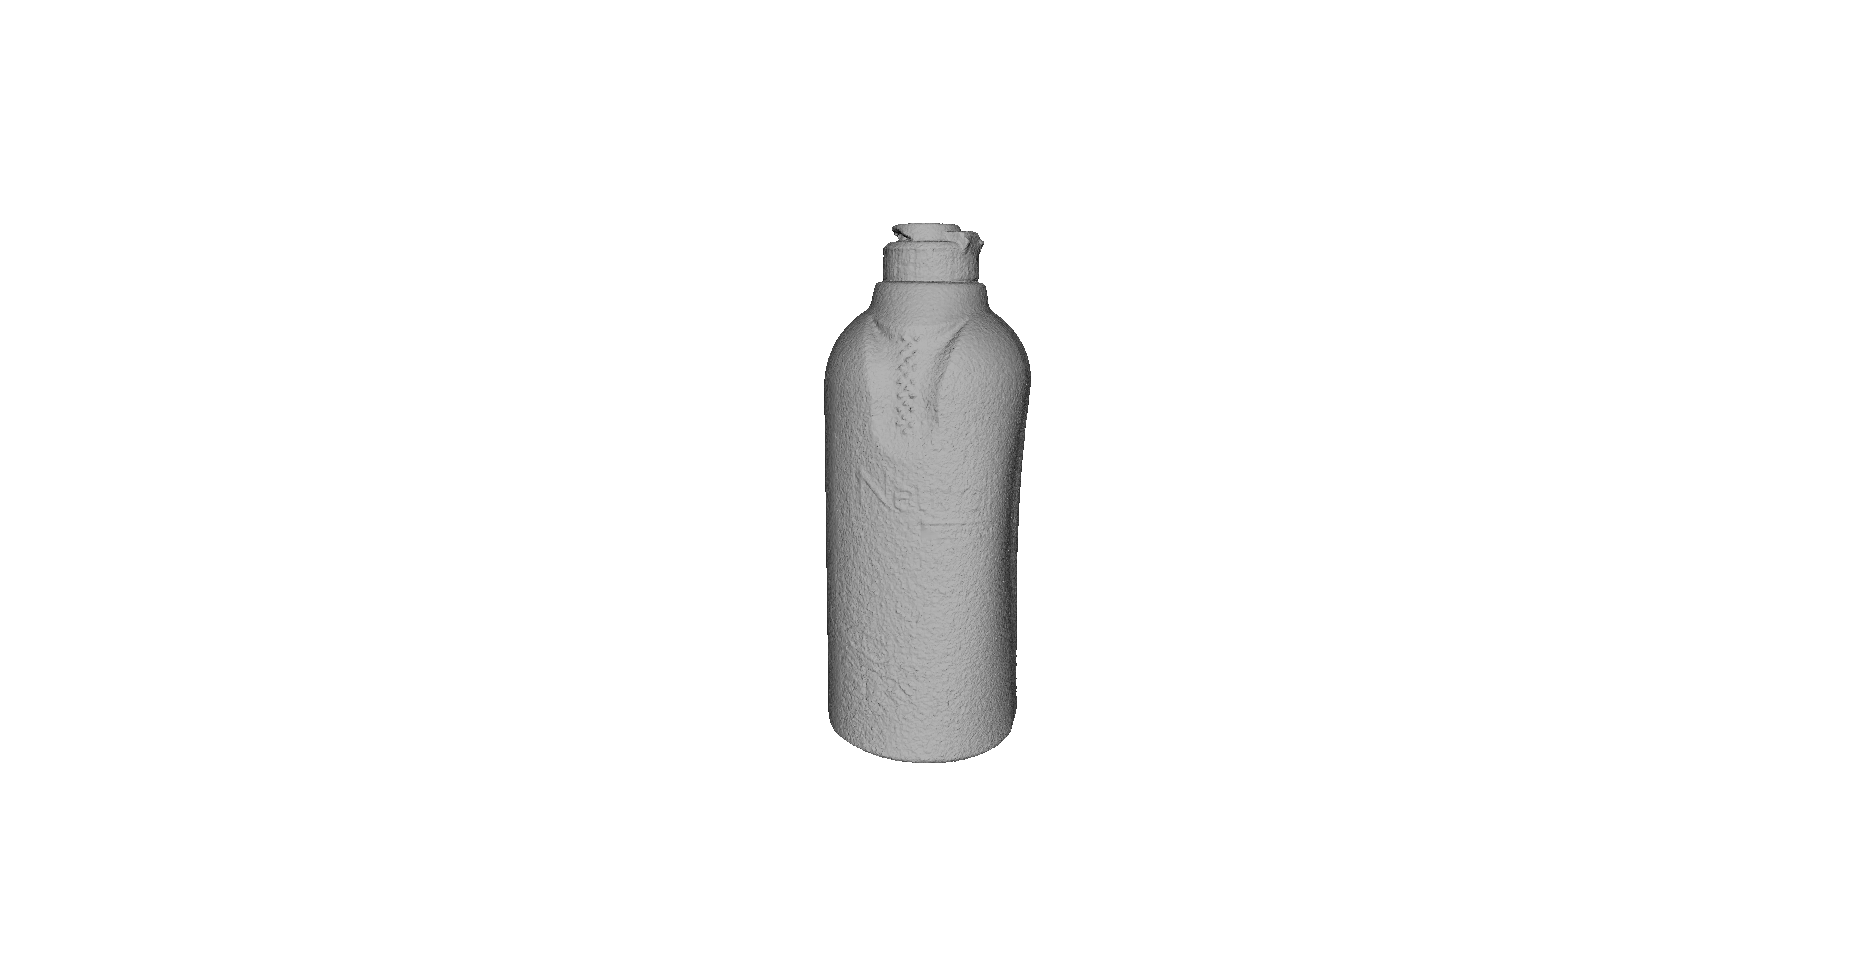
\includegraphics[clip, trim=12cm 2cm 12cm 2cm,width=0.12\linewidth, height= 0.12\linewidth, keepaspectratio]{img/snapshot08.png}
		%\caption{Noise level 3 for STL dataset}\label{fig:stl_n3}
		}
	\end{subfigure}
	\begin{subfigure}[Pringels]{%{.18\textwidth}
		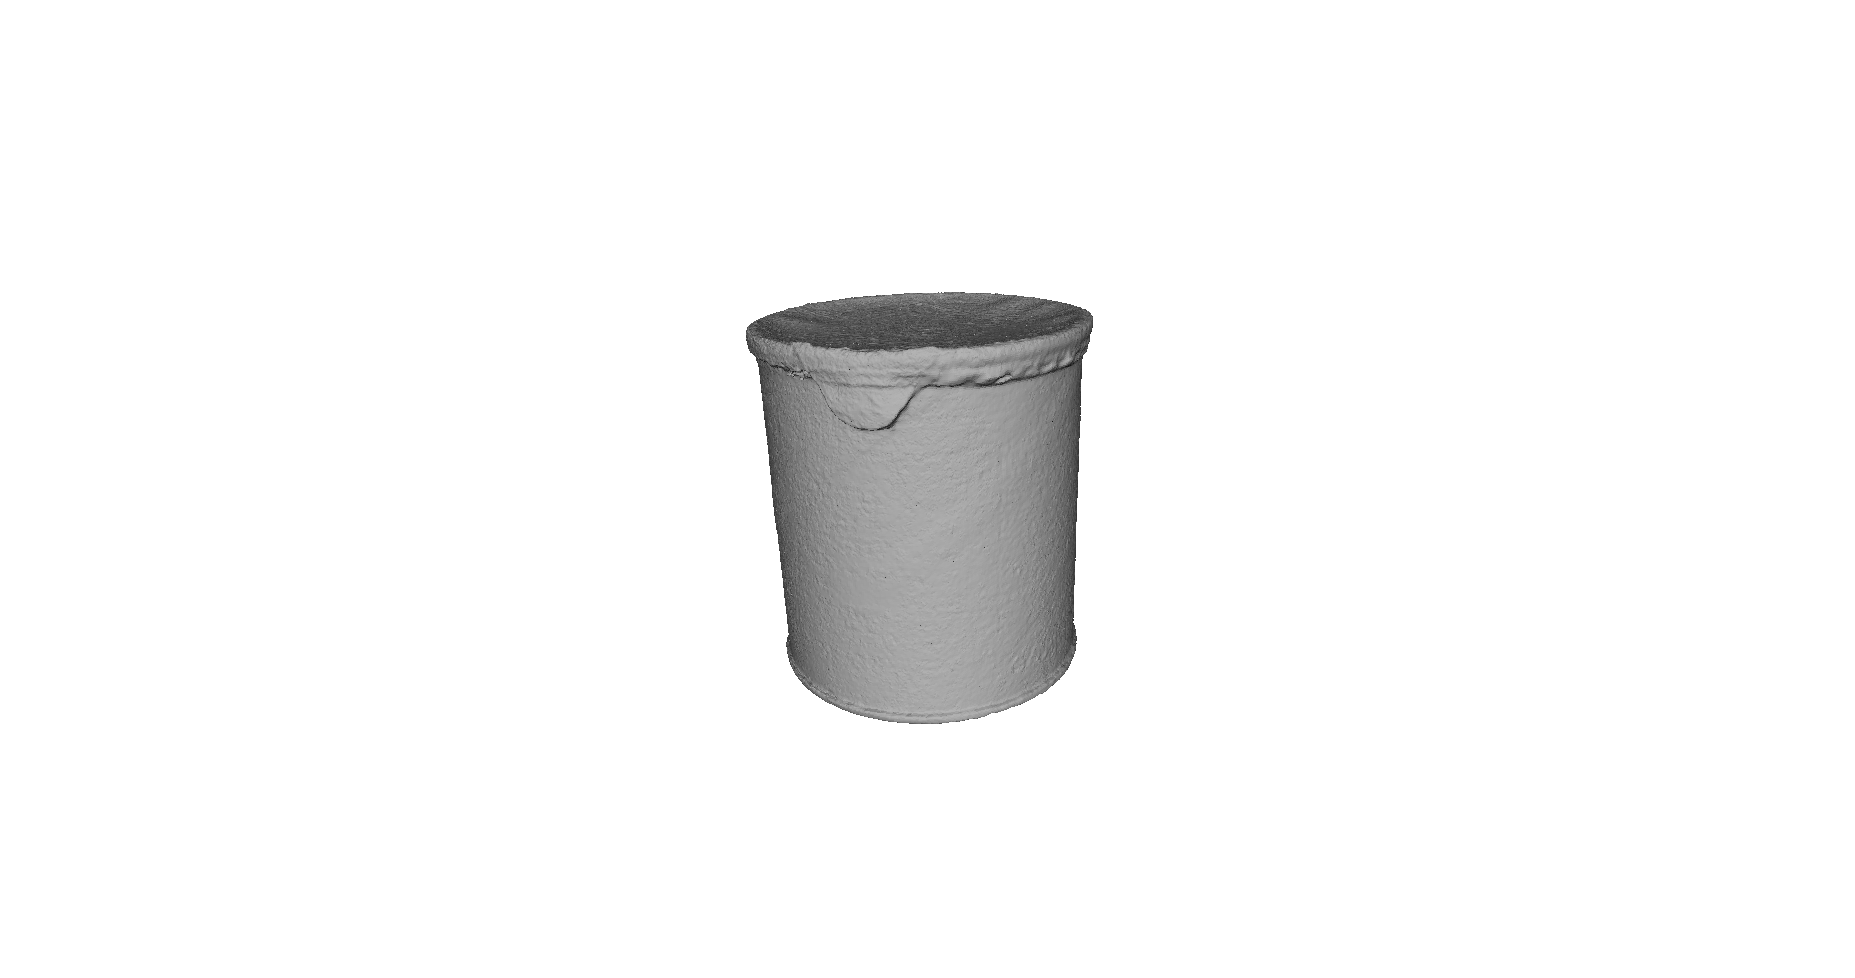
\includegraphics[clip, trim=12cm 2cm 12cm 2cm,width=0.12\linewidth, height= 0.12\linewidth, keepaspectratio]{img/snapshot14.png}
		%\caption{Noise level 3 for STL dataset}\label{fig:stl_n3}
		}
	\end{subfigure}
	\\
	\begin{subfigure}[Hand soap]{%{.18\textwidth}
		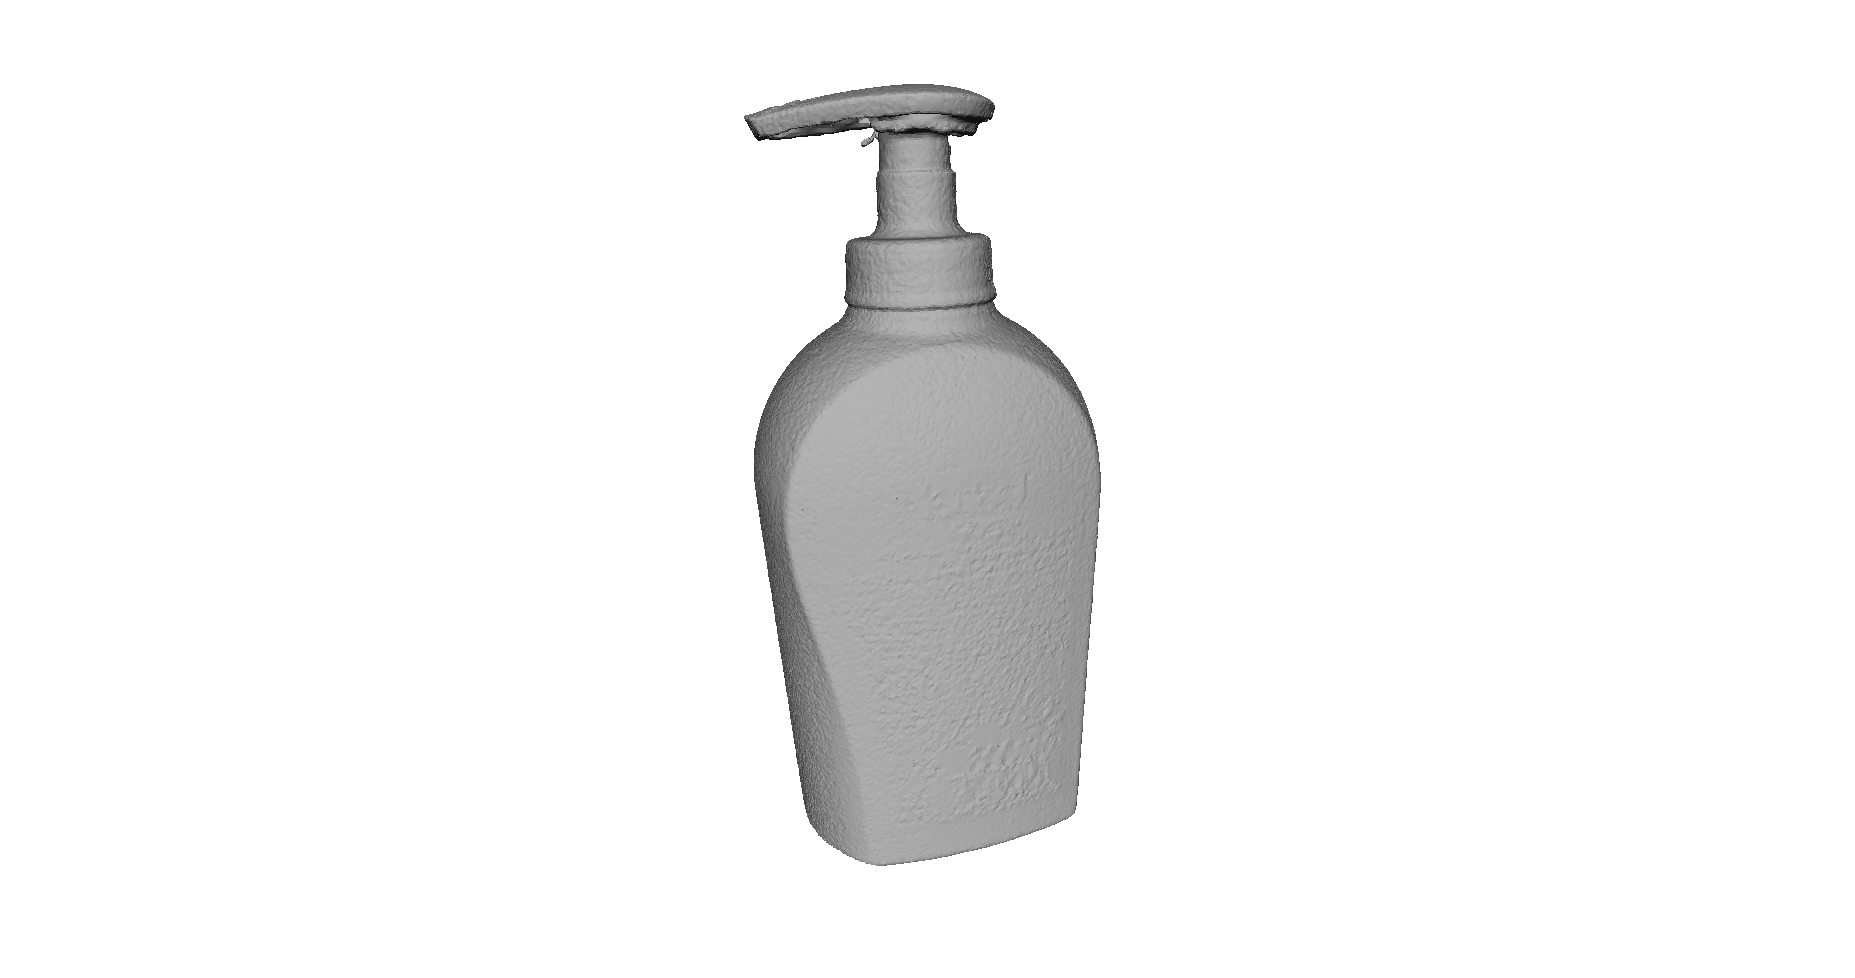
\includegraphics[clip, trim=12cm 2cm 12cm 2cm,width=0.12\linewidth, height= 0.12\linewidth, keepaspectratio]{img/snapshot17.png}
		%\caption{Noise level 3 for STL dataset}\label{fig:stl_n3}
		}
	\end{subfigure}
	\begin{subfigure}[Button]{%{.18\textwidth}
		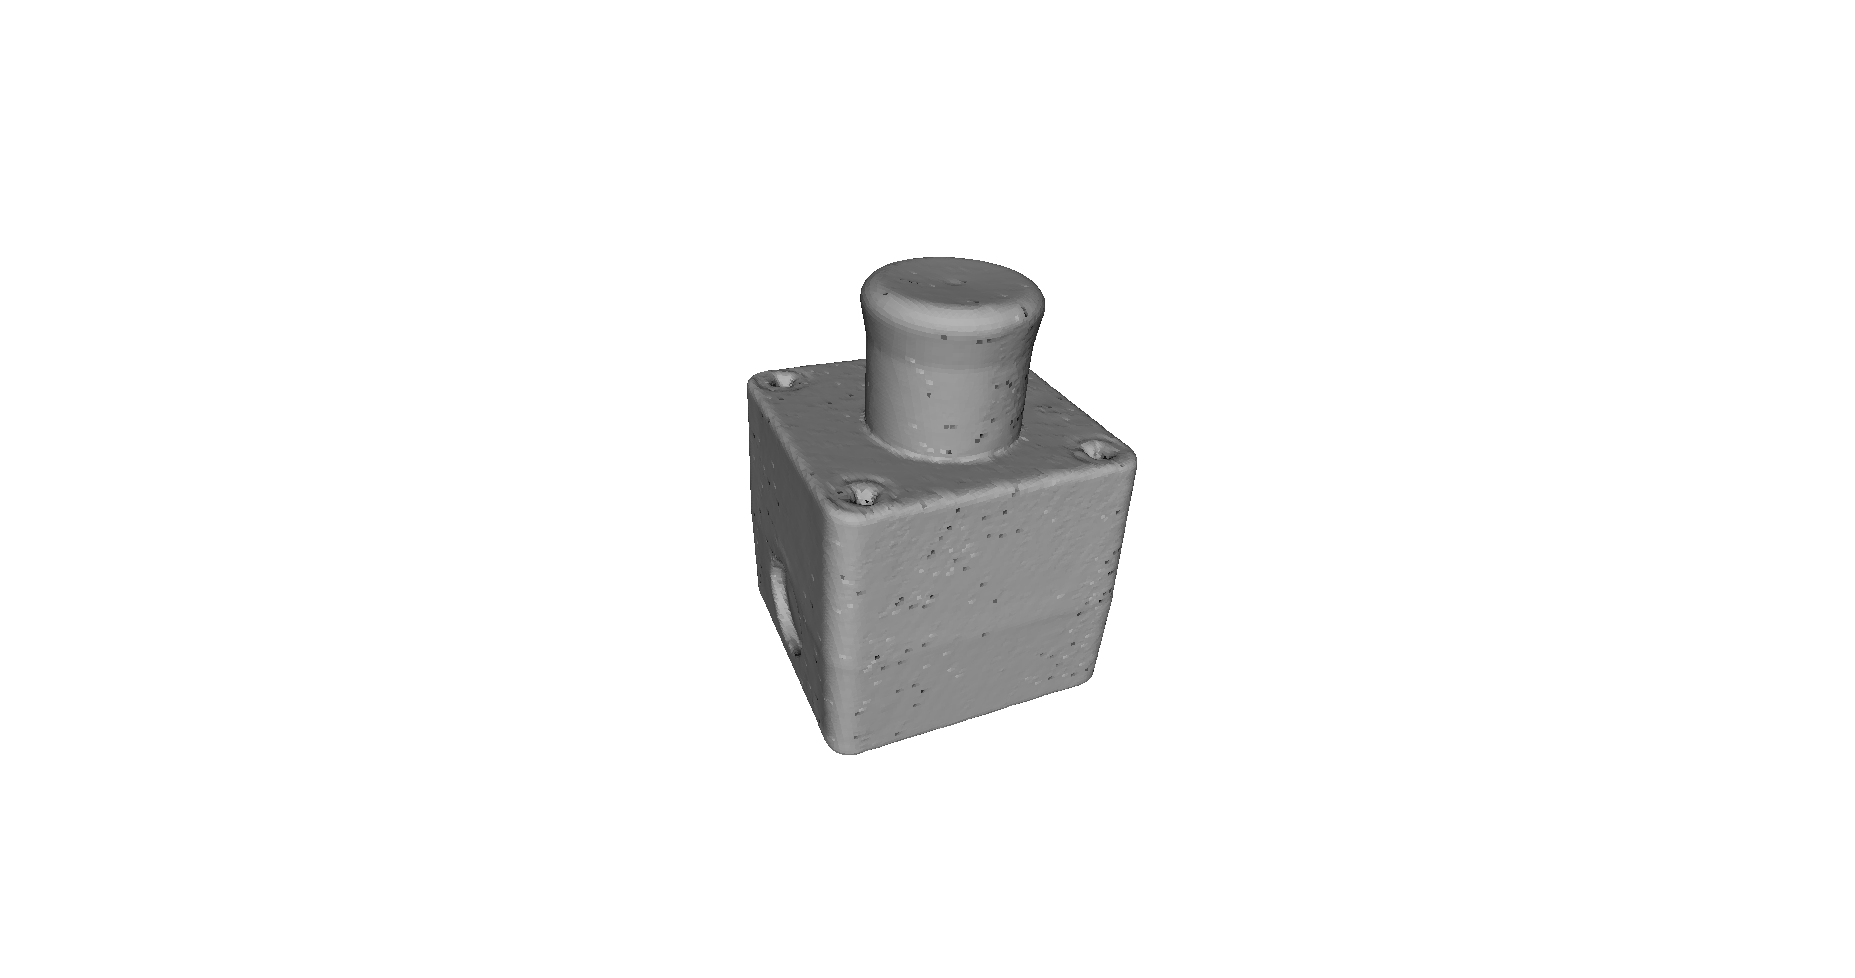
\includegraphics[clip, trim=12cm 2cm 12cm 2cm,width=0.12\linewidth, height= 0.12\linewidth, keepaspectratio]{img/snapshot22.png}
		%\caption{Noise level 3 for STL dataset}\label{fig:stl_n3}
		}
	\end{subfigure}
	\begin{subfigure}[Brake disc]{%{.18\textwidth}
		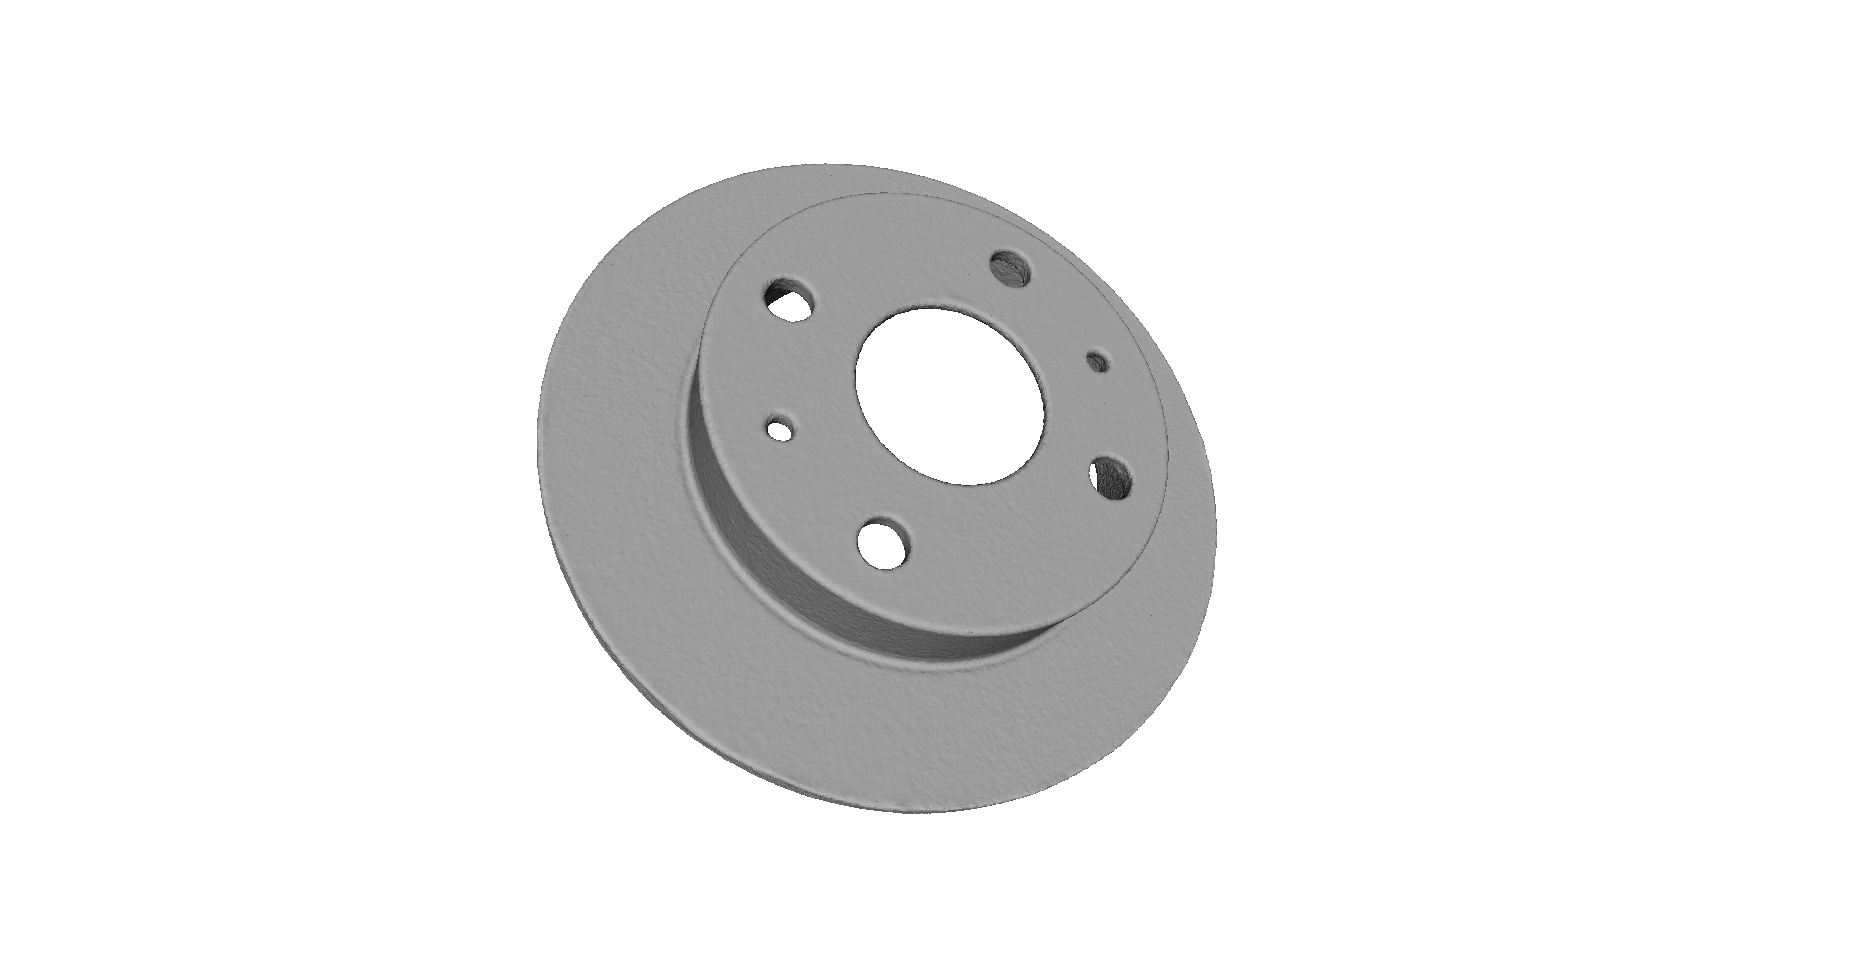
\includegraphics[clip, trim=12cm 2cm 12cm 2cm,width=0.12\linewidth, height= 0.12\linewidth, keepaspectratio]{img/snapshot40.png}
		%\caption{Noise level 3 for STL dataset}\label{fig:stl_n3}
		}
	\end{subfigure}
	\begin{subfigure}[Psu]{%{.18\textwidth}
		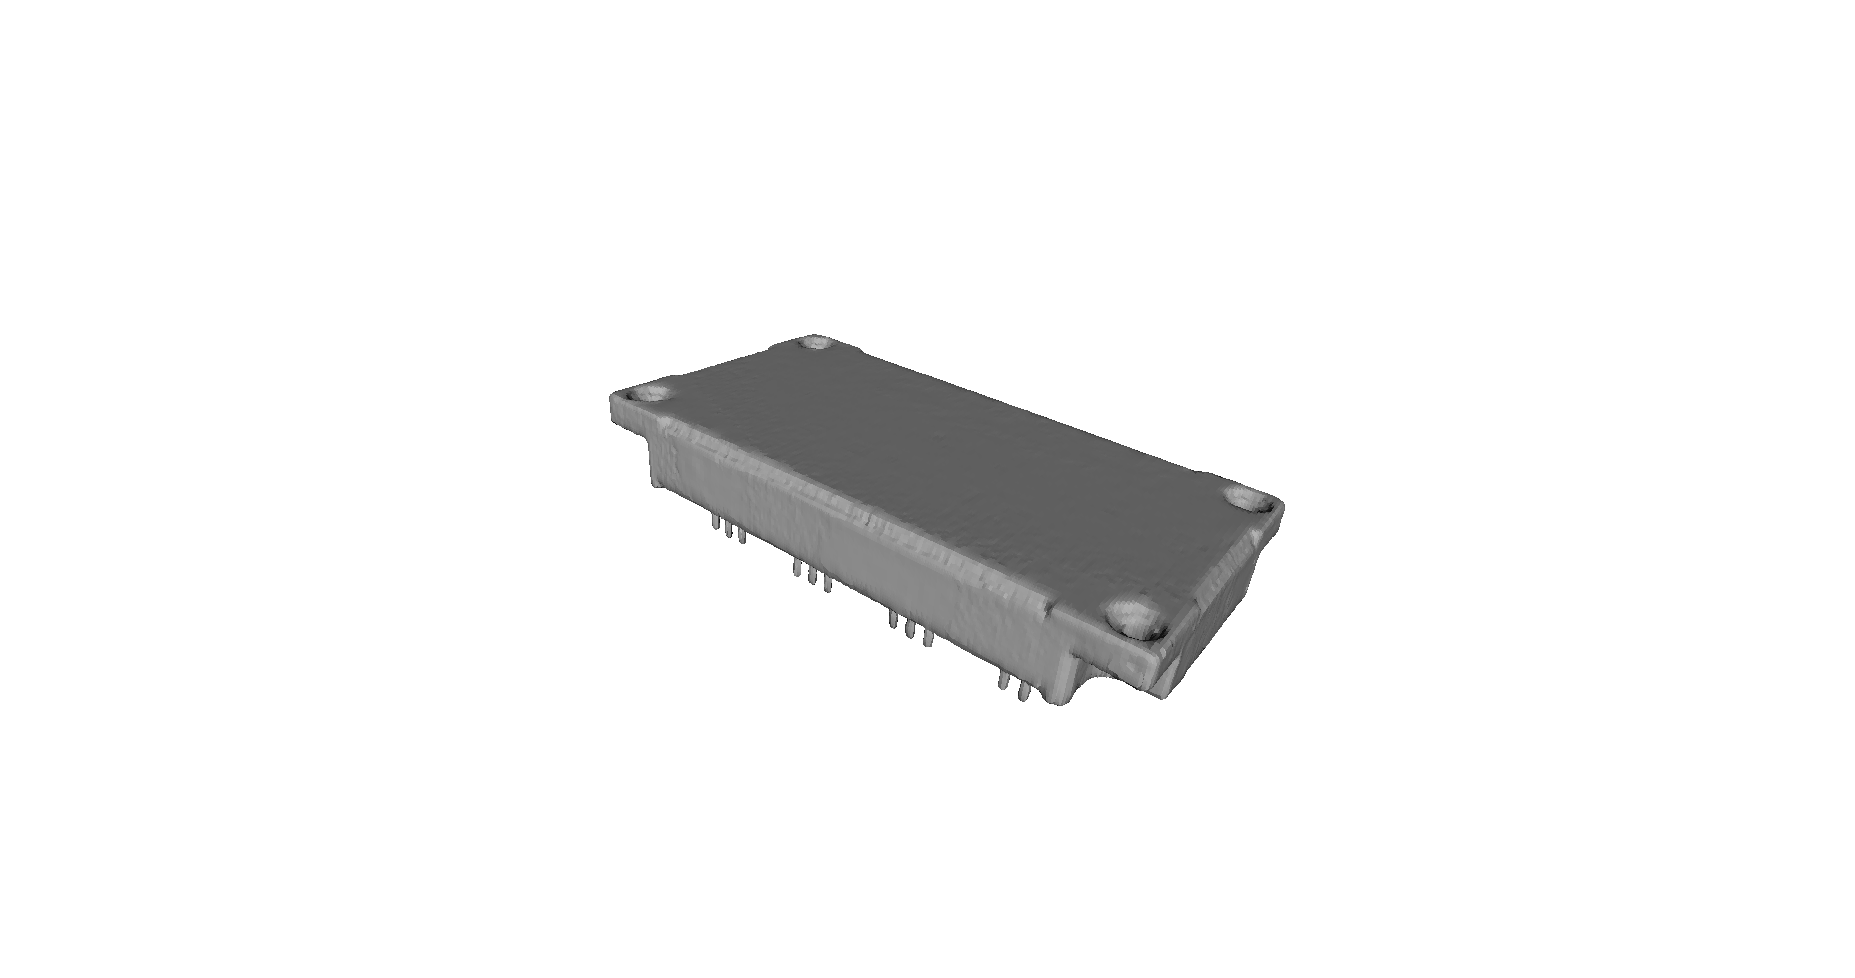
\includegraphics[clip, trim=12cm 2cm 12cm 2cm,width=0.12\linewidth, height= 0.12\linewidth, keepaspectratio]{img/snapshot24.png}
		%\caption{Noise level 3 for STL dataset}\label{fig:stl_n3}
		}
	\end{subfigure}
	\captionsetup{justification=centering}
\caption{(a)-(c) Geometric complex objects used for dataset verification. (d)-(e) Cylinderical objects local. (f)-(h) Flat and box shaped objects}\label{fig:selected_objects}
\end{figure*}

\begin{figure*}[h]
\begin{minipage}[b]{.3\textwidth}
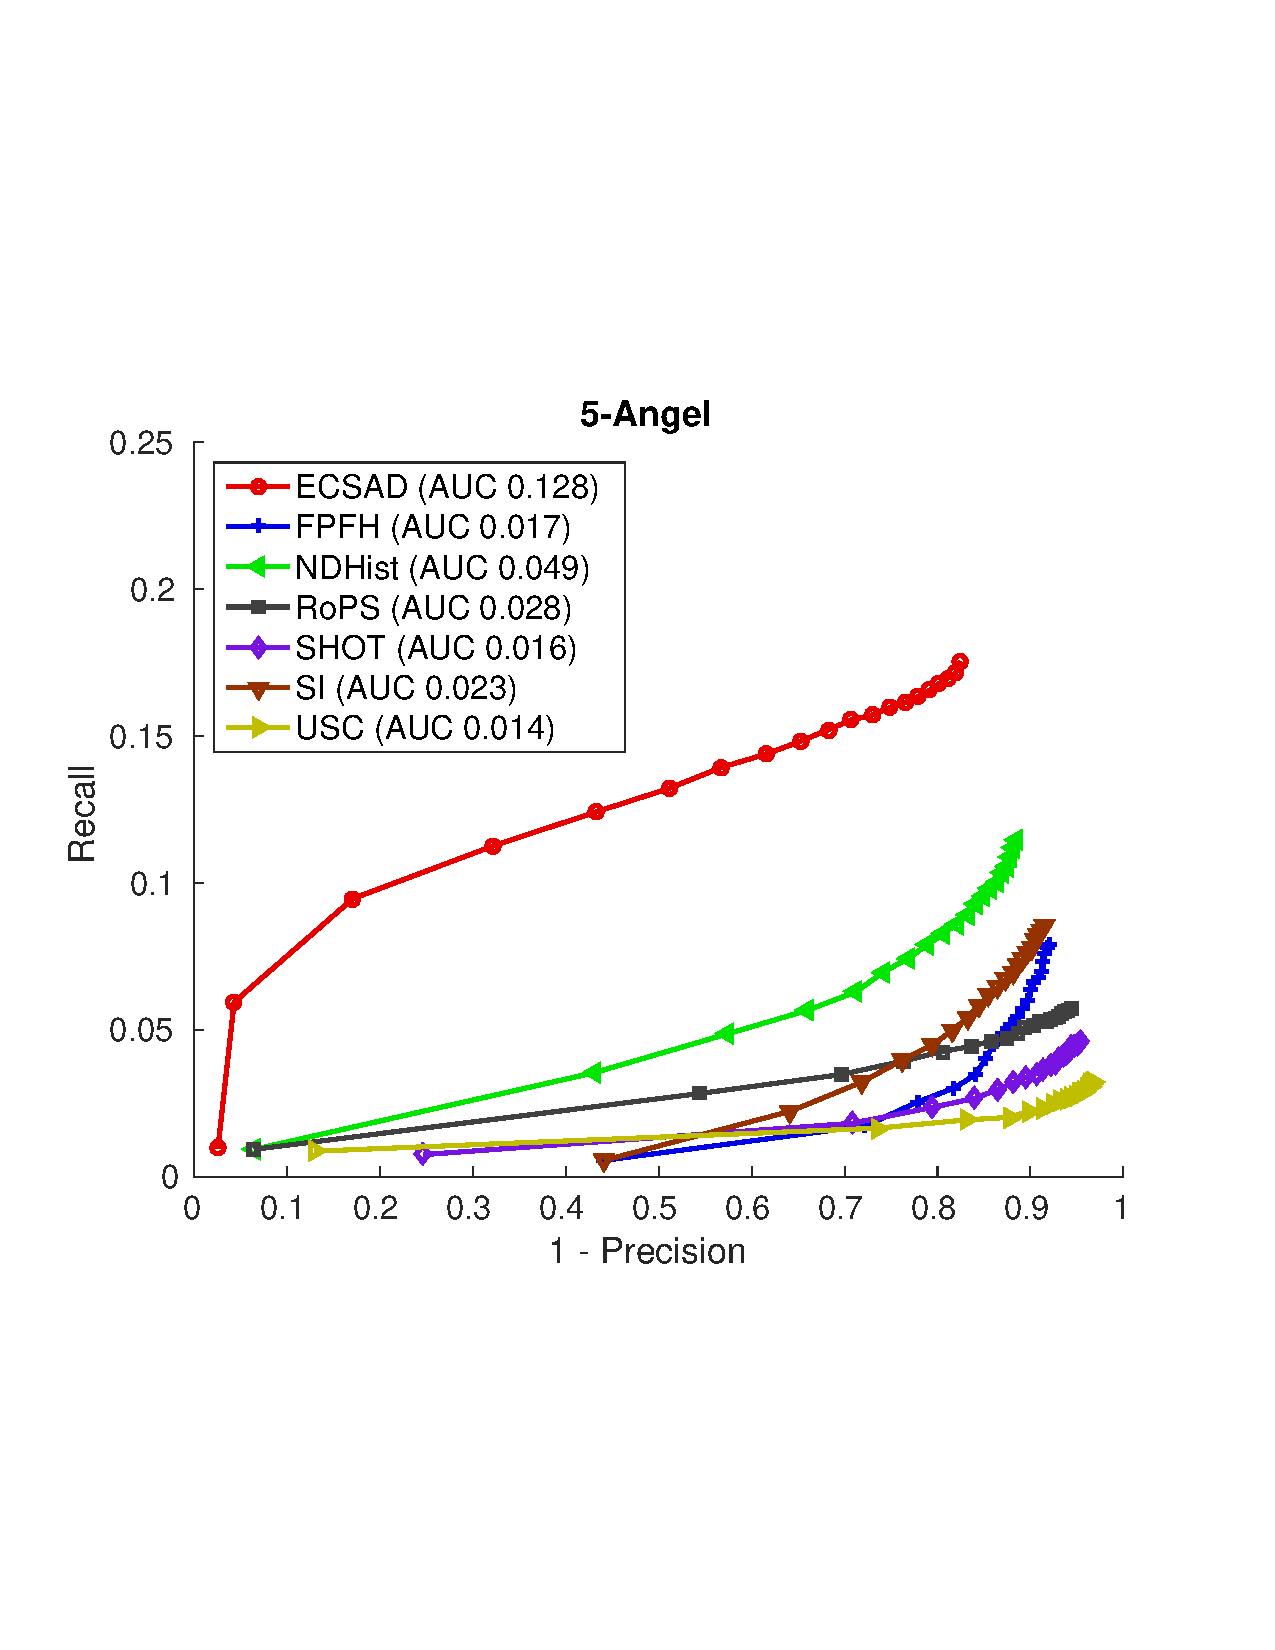
\includegraphics[clip, trim=0.7cm 6cm 0.7cm 6cm,width=1.0\linewidth, height= 1.0\linewidth, keepaspectratio]{img/5-Angel_L2_RATIO_zoom.pdf} 
\caption{PRC curve: Angel }\label{fig:angel}
\end{minipage}\qquad
\begin{minipage}[b]{.3\textwidth}
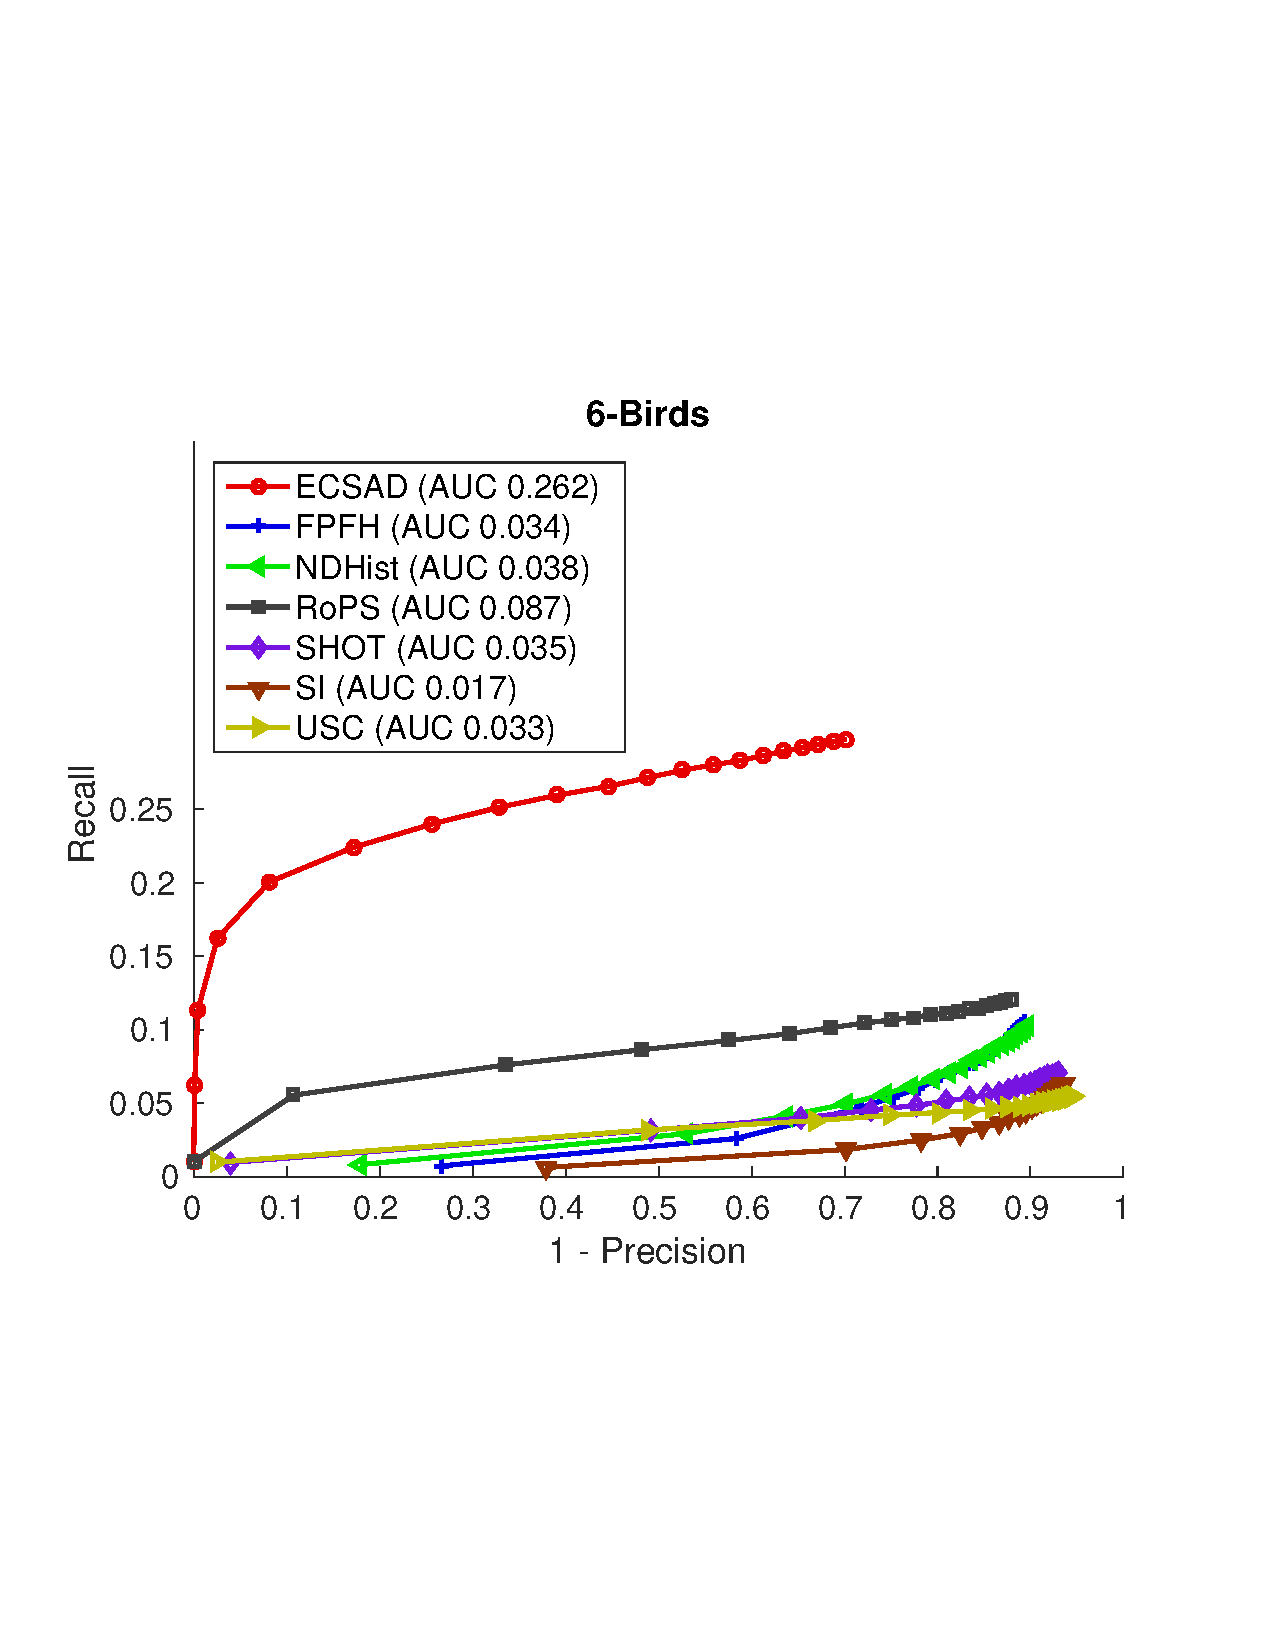
\includegraphics[clip, trim=0.7cm 6cm 0.7cm 6cm,width=1.0\linewidth, height= 1.0\linewidth, keepaspectratio]{img/6-Birds_L2_RATIO_zoom.pdf}
\caption{PRC curve: Birds }\label{fig:birds}
\end{minipage}
\begin{minipage}[b]{.3\textwidth}
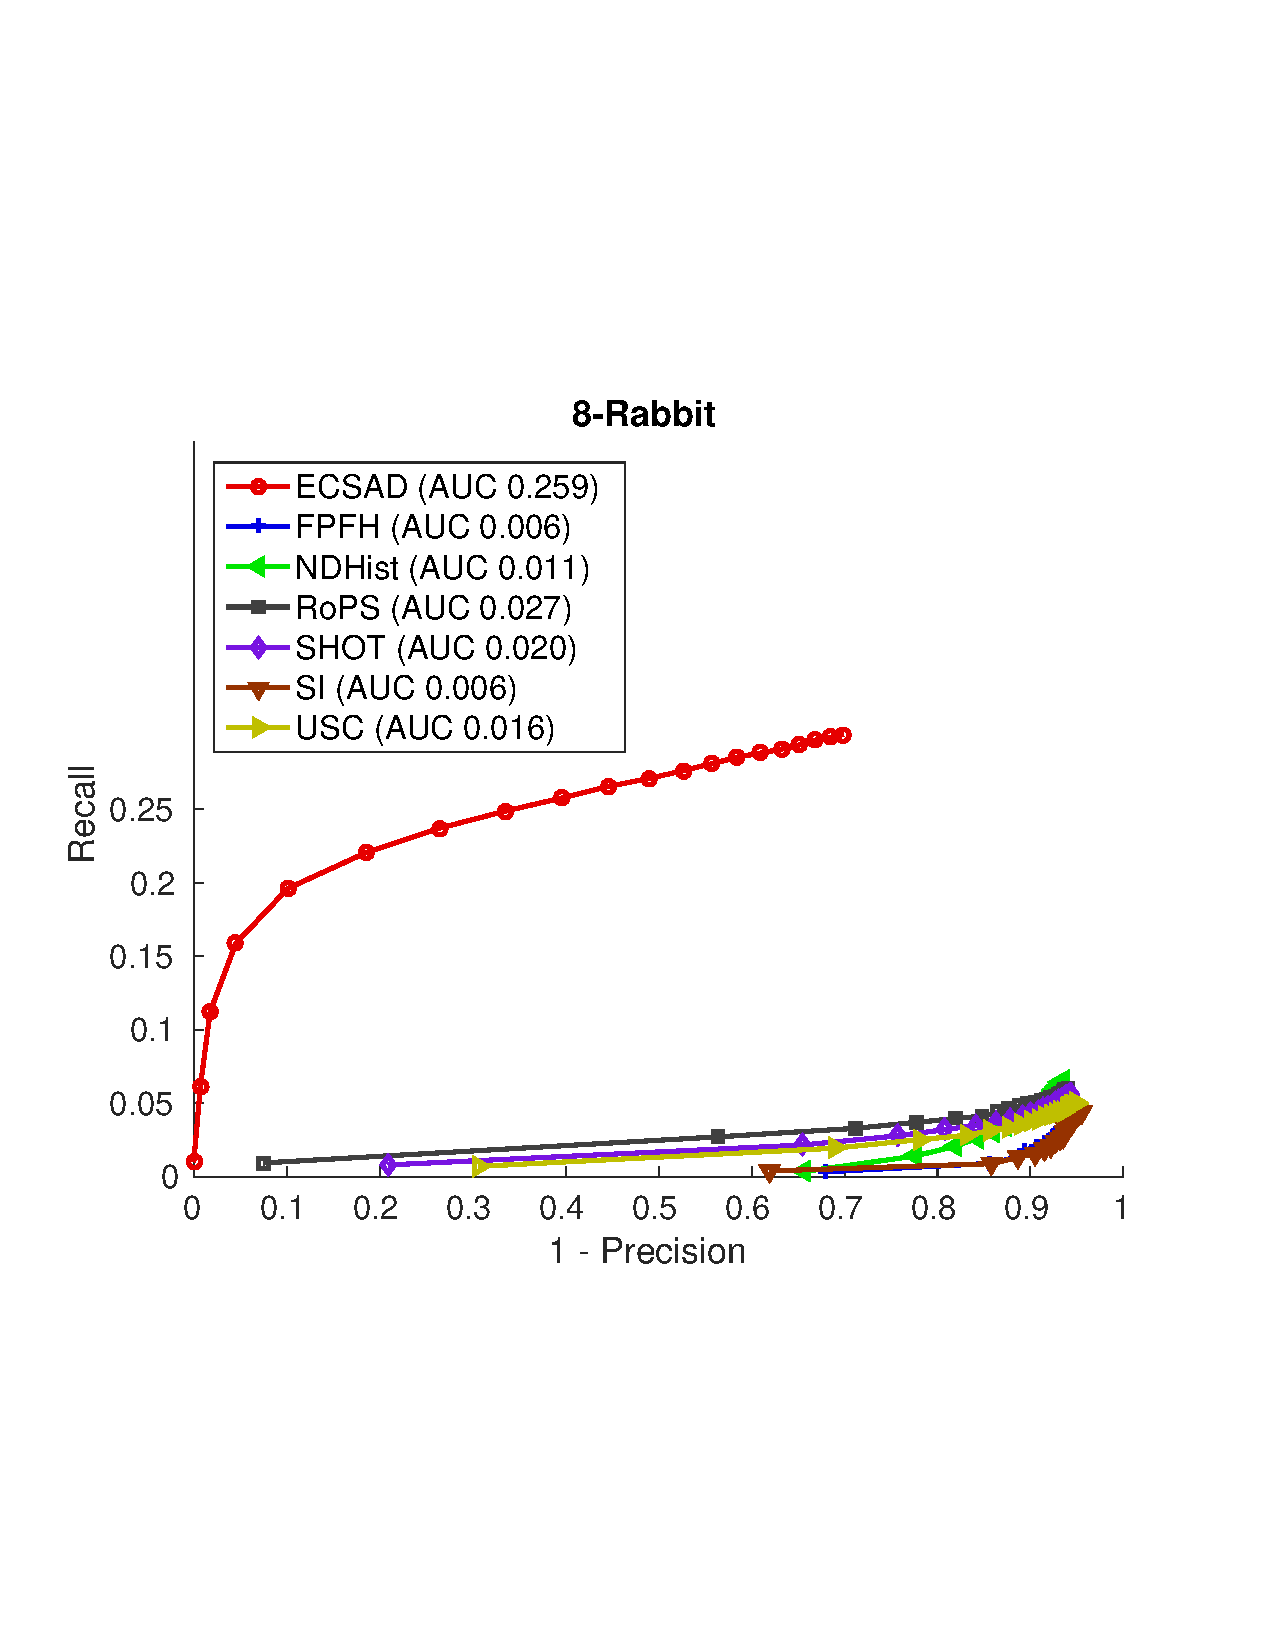
\includegraphics[clip, trim=0.7cm 6cm 0.7cm 6cm,width=1.0\linewidth, height= 1.0\linewidth, keepaspectratio]{img/8-Rabbit_L2_RATIO_zoom.pdf}
\caption{PRC curve: Rabbit }\label{fig:rabbit}
\end{minipage}
\end{figure*}

\begin{figure*}[h]
\begin{minipage}[b]{.3\textwidth}
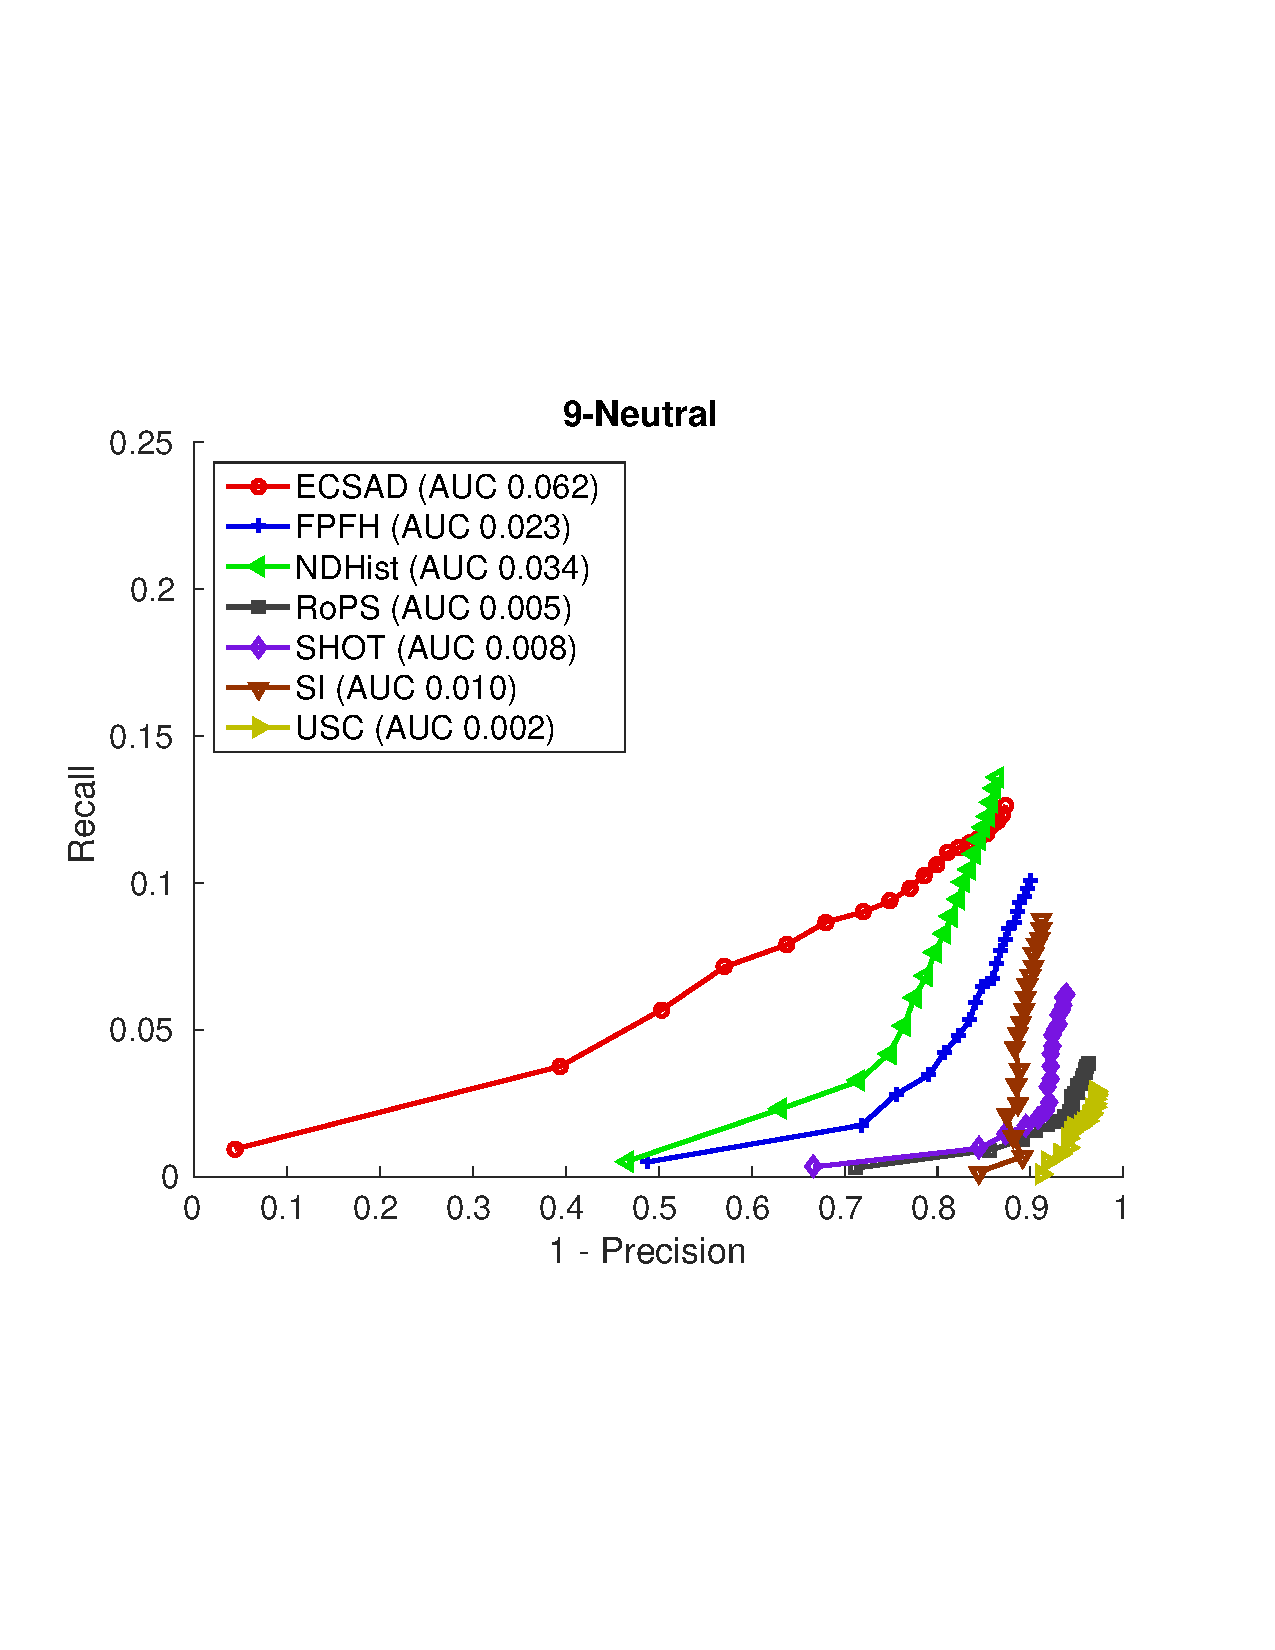
\includegraphics[clip, trim=0.7cm 6cm 0.7cm 6cm,width=1.0\linewidth, height= 1.0\linewidth, keepaspectratio]{img/9-Neutral_L2_RATIO_zoom.pdf} 
\caption{PRC curve: Neutral }\label{fig:neutral}
\end{minipage}\qquad
\begin{minipage}[b]{.3\textwidth}
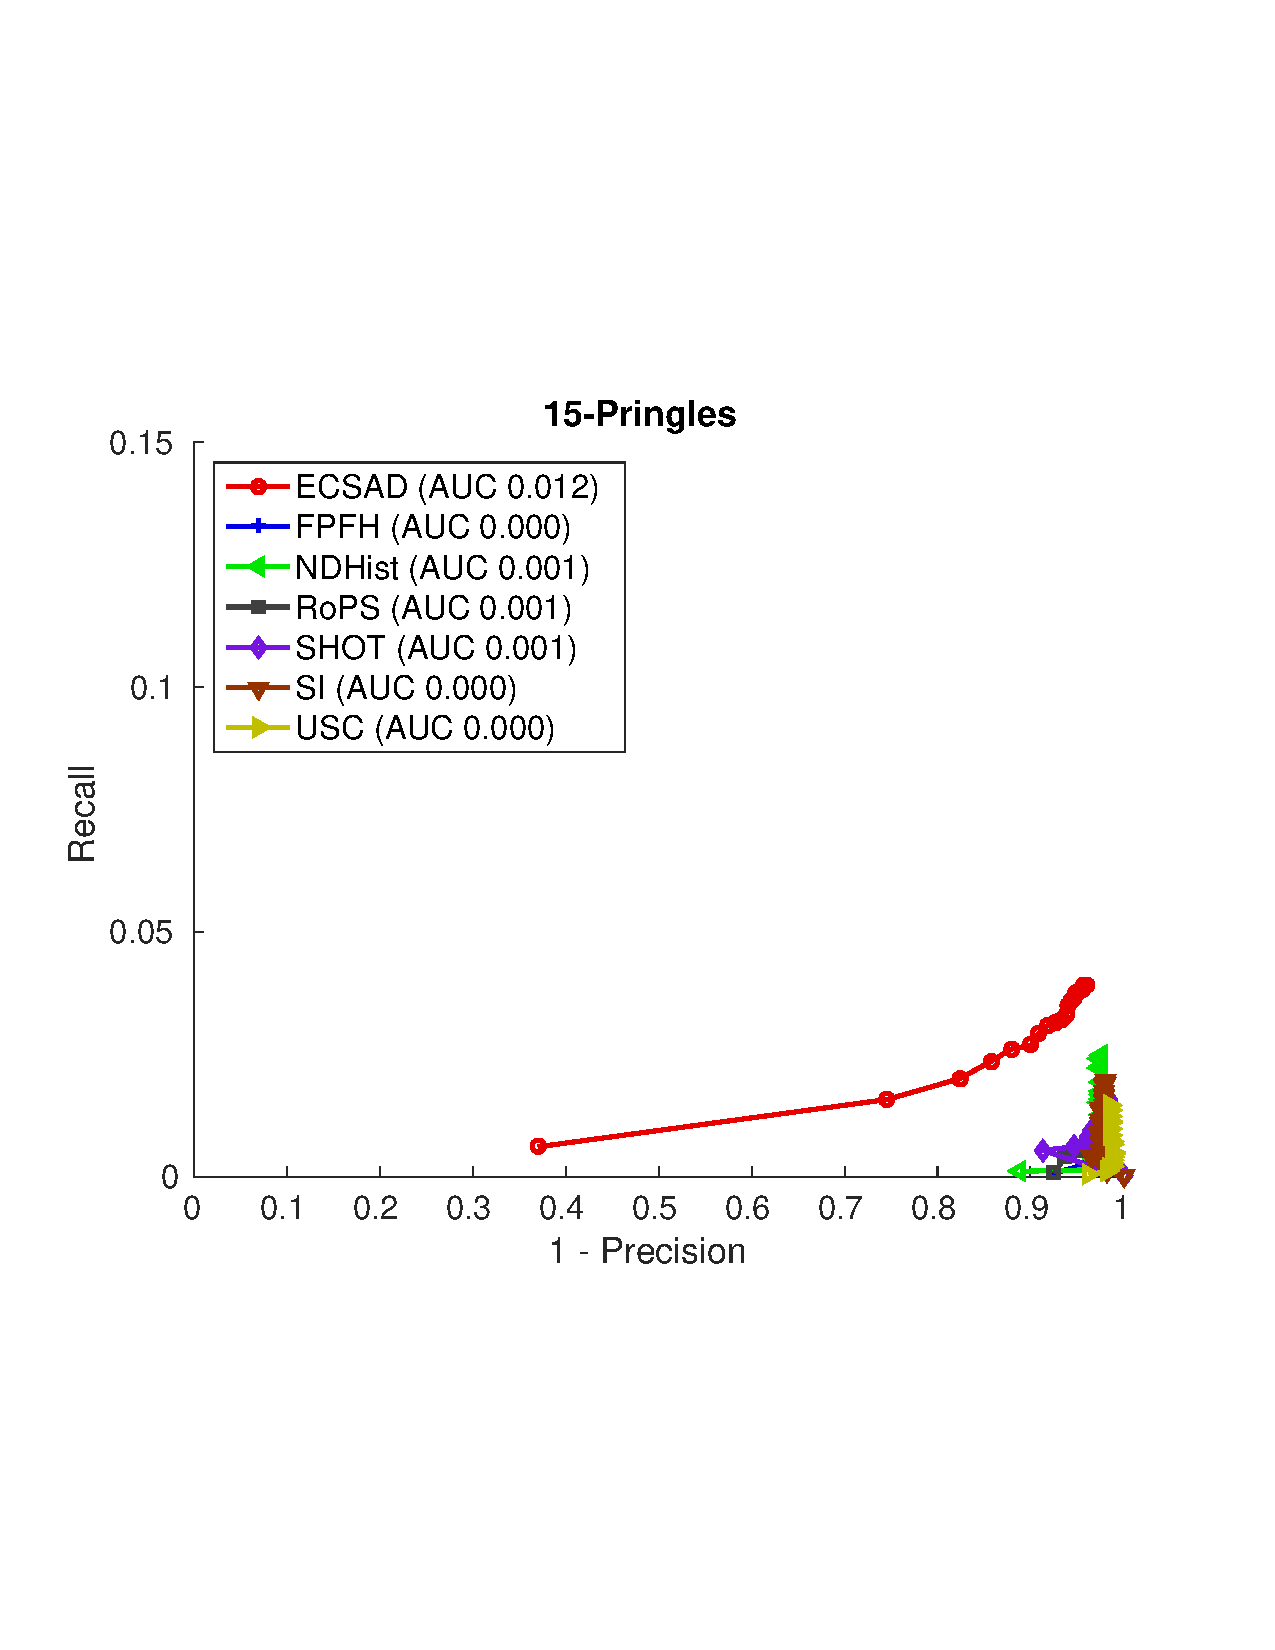
\includegraphics[clip, trim=0.7cm 6cm 0.7cm 6cm,width=1.0\linewidth, height= 1.0\linewidth, keepaspectratio]{img/15-Pringles_L2_RATIO_zoom.pdf}
\caption{PRC curve: Pringles}\label{fig:pringles}
\end{minipage}
\begin{minipage}[b]{.3\textwidth}
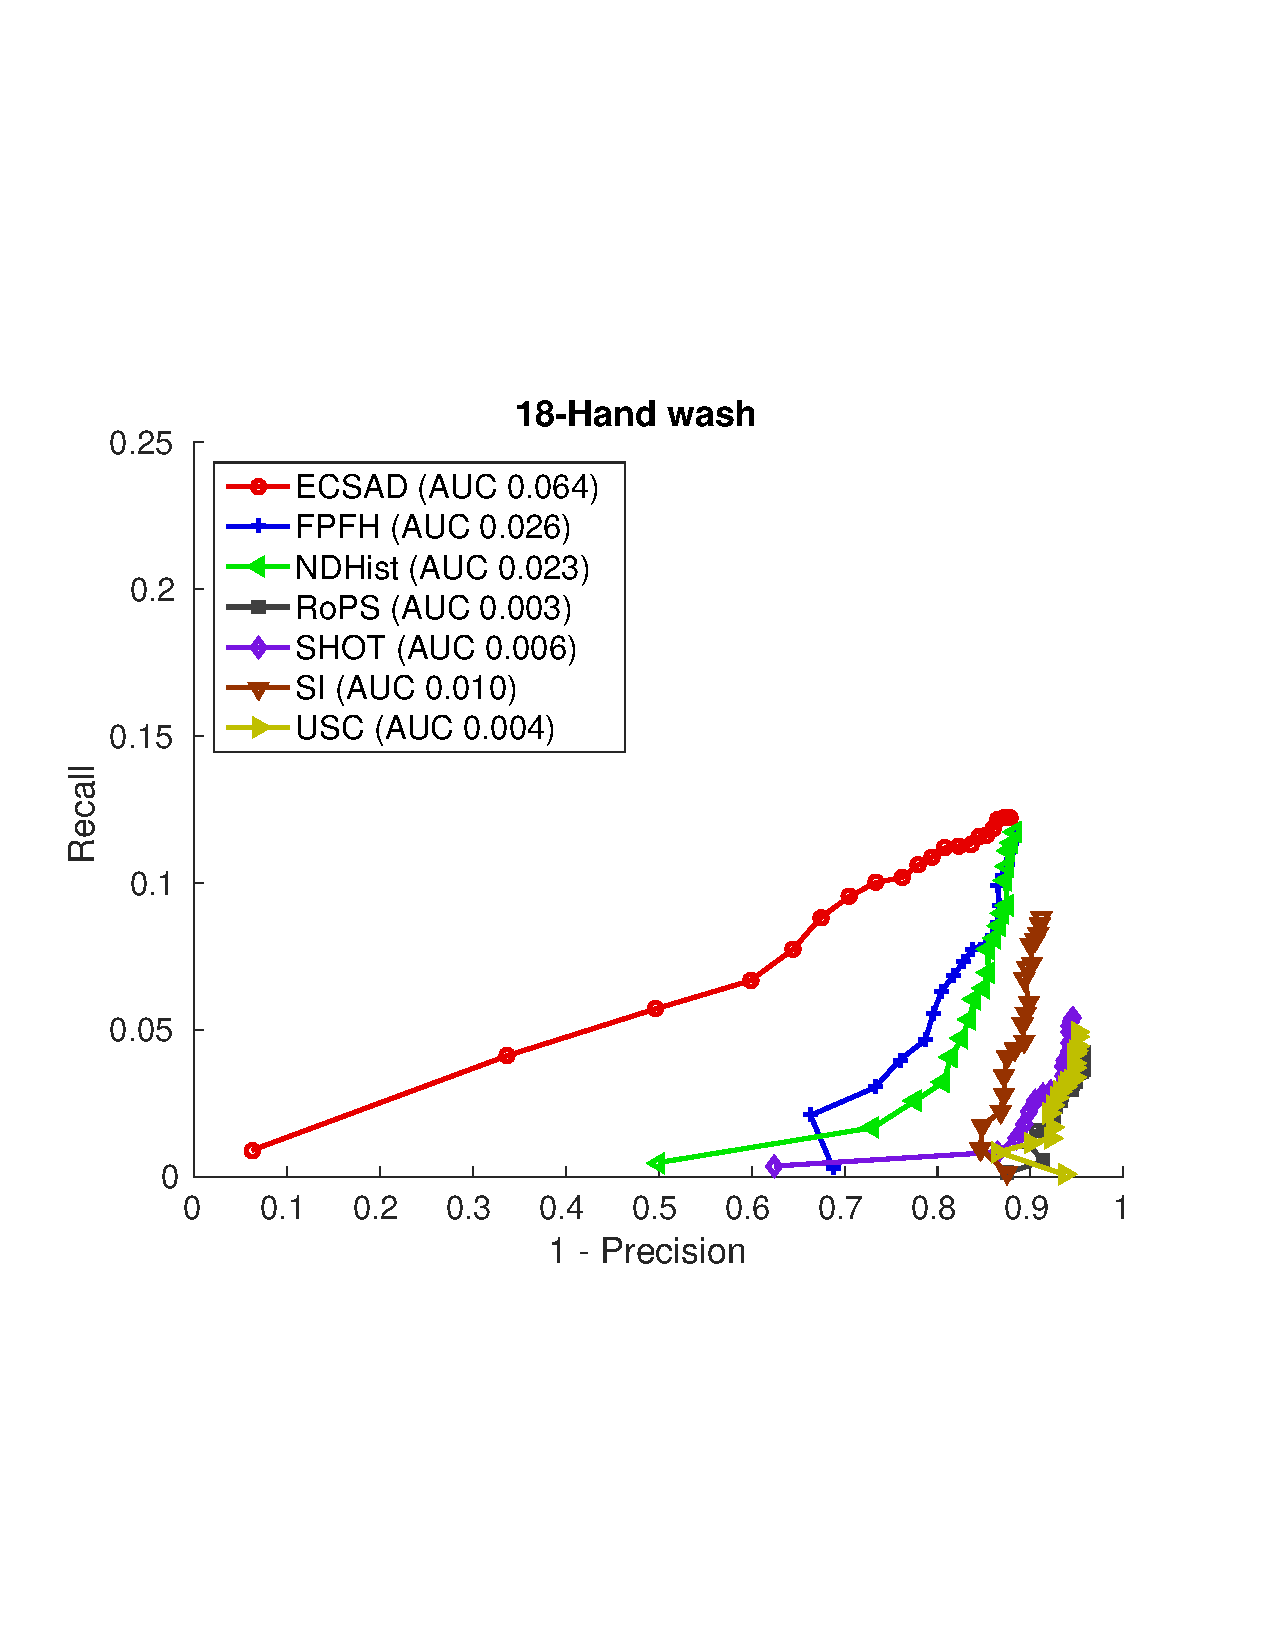
\includegraphics[clip, trim=0.7cm 6cm 0.7cm 6cm,width=1.0\linewidth, height= 1.0\linewidth, keepaspectratio]{img/18-Hand_wash_L2_RATIO_zoom.pdf}
\caption{PRC curve: Hand soap}\label{fig:hand_soap}
\end{minipage}
\end{figure*}

\begin{figure*}[h]
\begin{minipage}[b]{.3\textwidth}
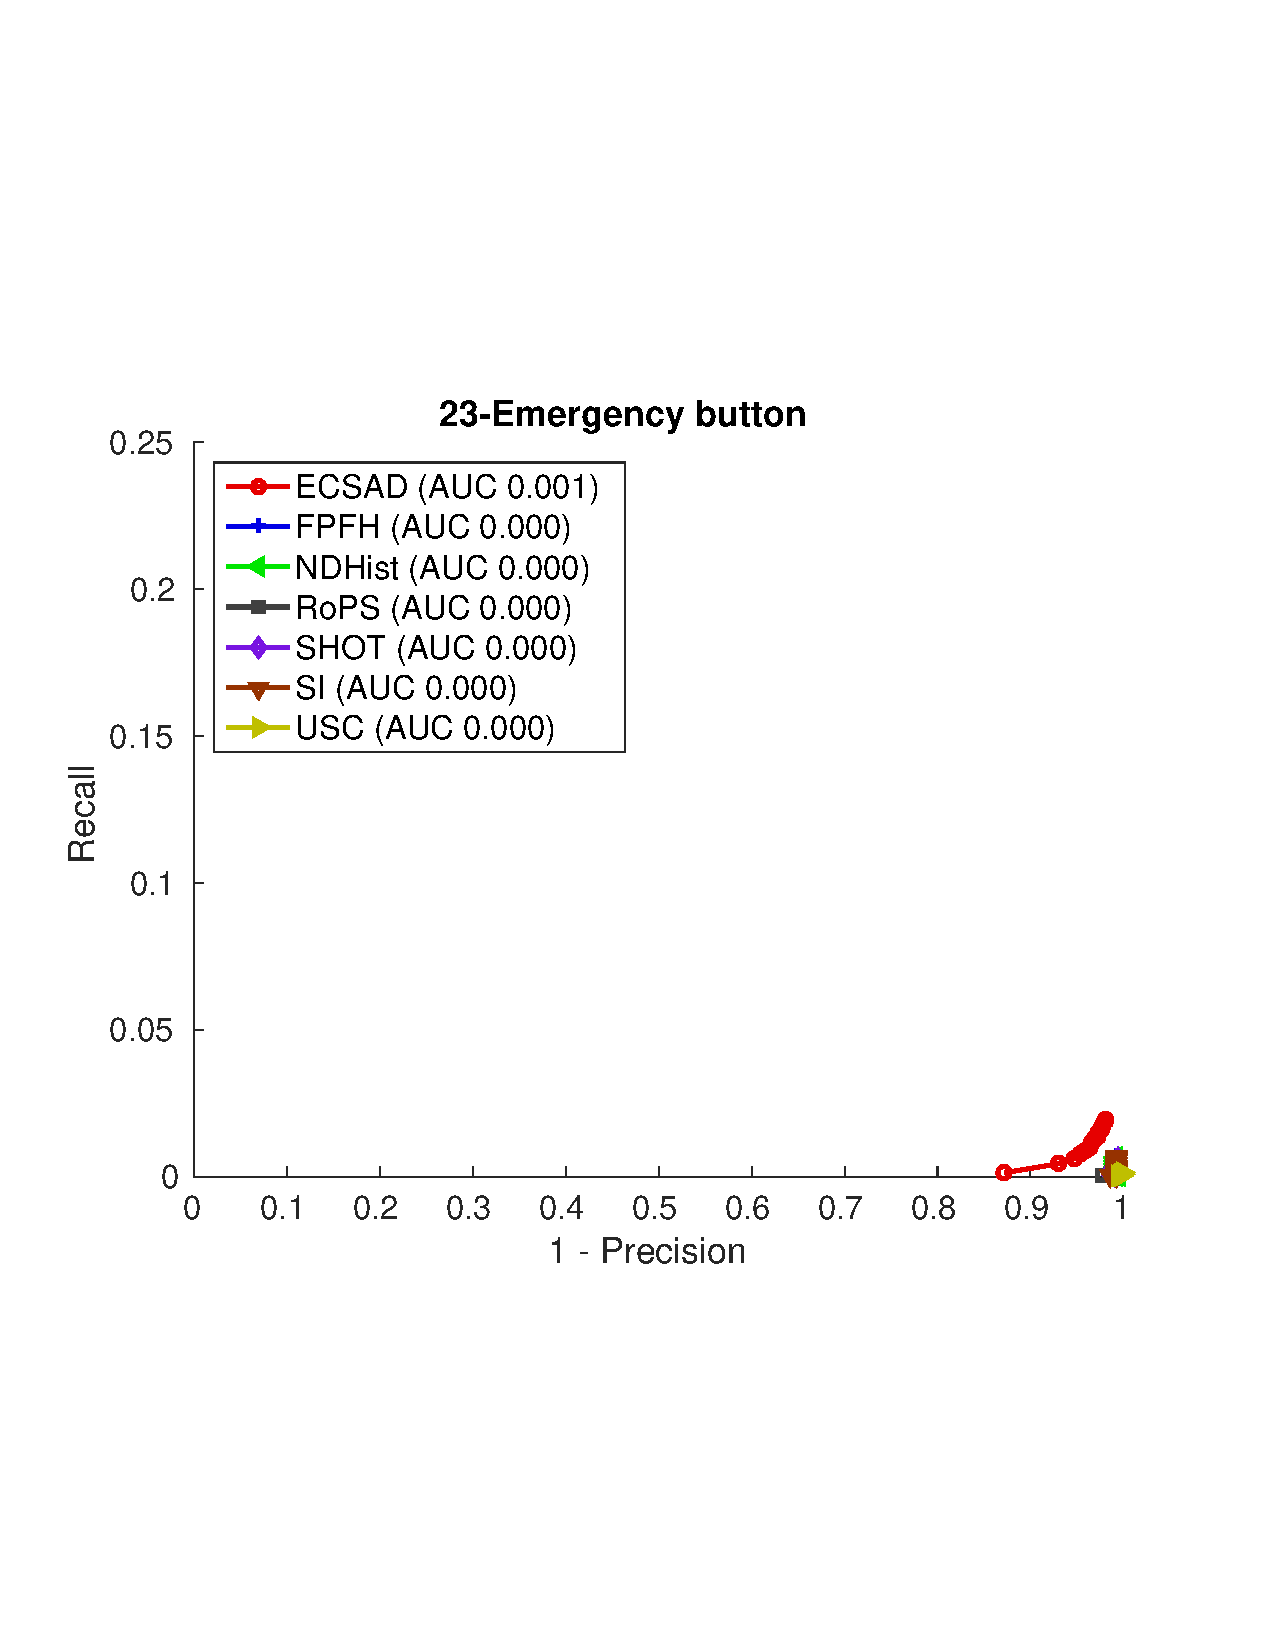
\includegraphics[clip, trim=0.7cm 6cm 0.7cm 6cm,width=1.0\linewidth, height= 1.0\linewidth, keepaspectratio]{img/23-Emergency_button_L2_RATIO_zoom.pdf} 
\caption{PRC curve: Button }\label{fig:button}
\end{minipage}\qquad
\begin{minipage}[b]{.3\textwidth}
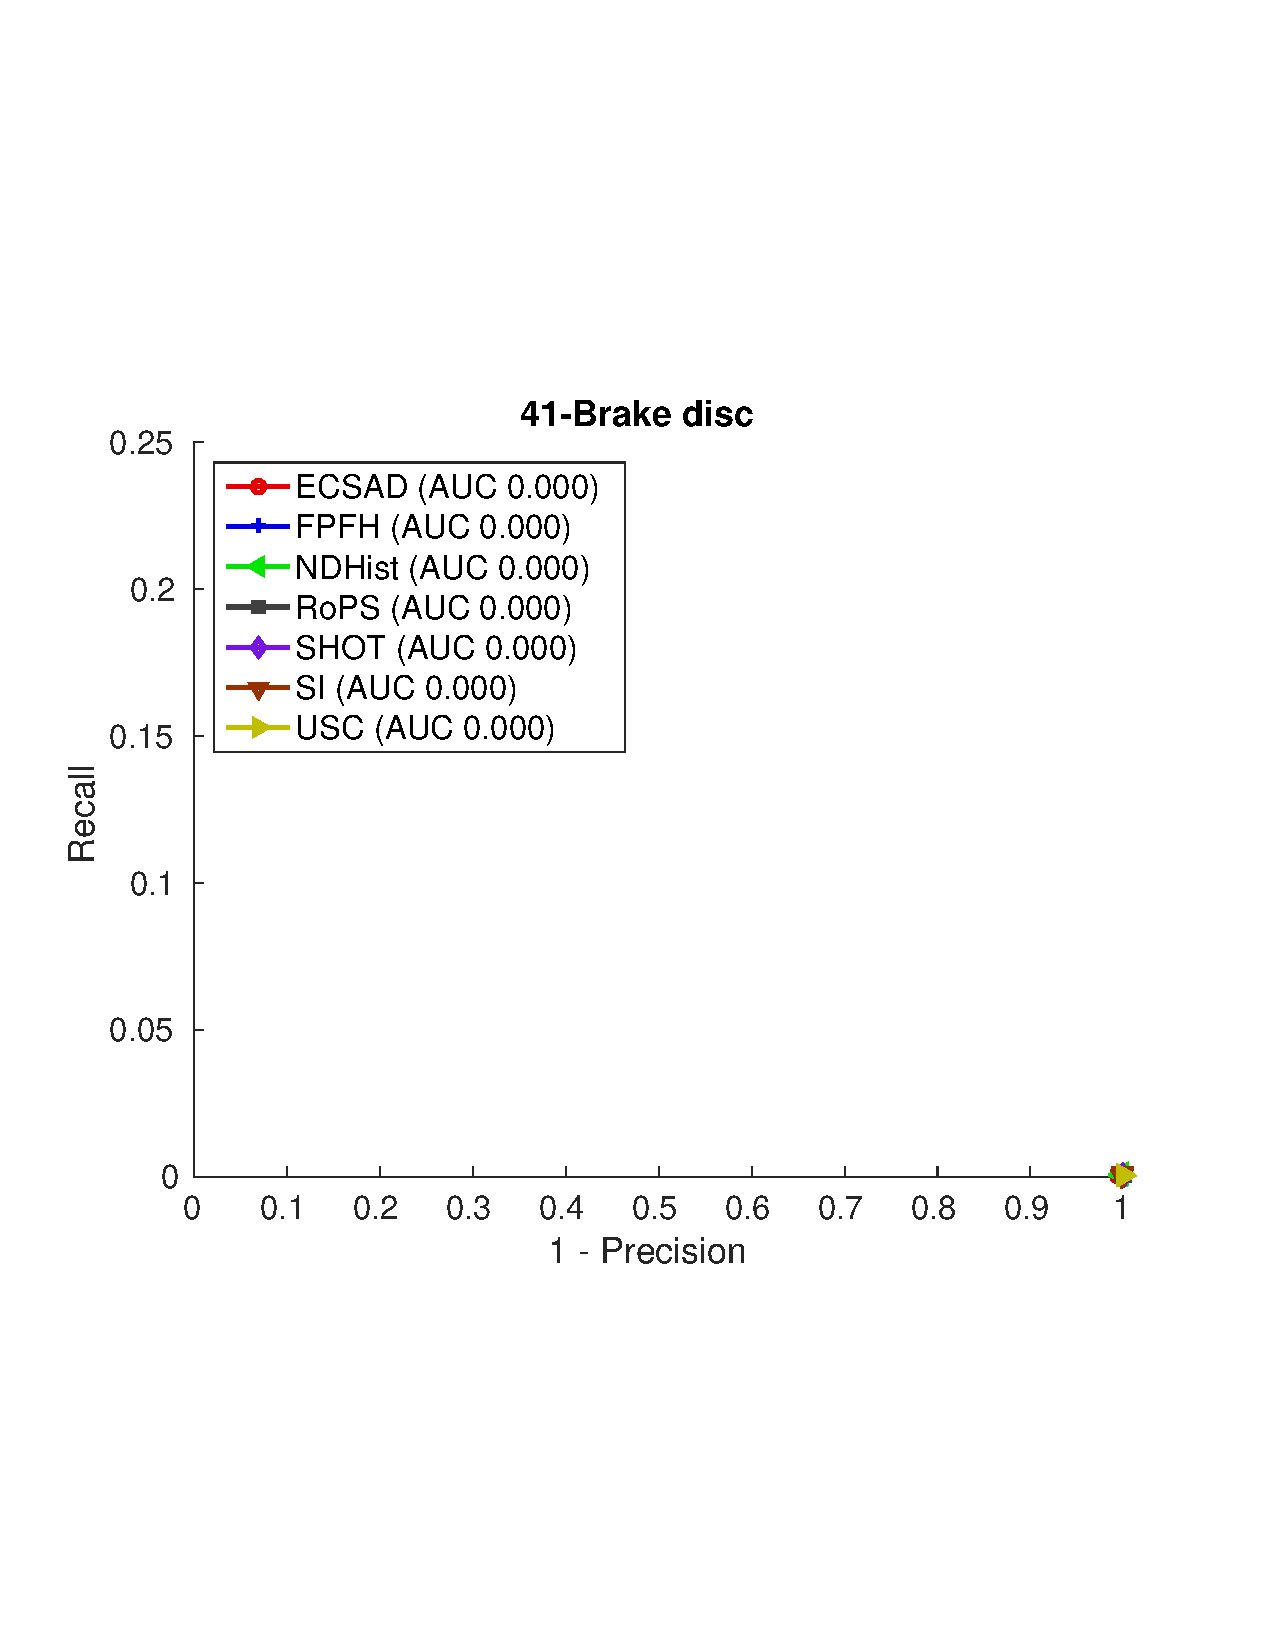
\includegraphics[clip, trim=0.7cm 6cm 0.7cm 6cm,width=1.0\linewidth, height= 1.0\linewidth, keepaspectratio]{img/41-Brake_disc_L2_RATIO_zoom.pdf}
\caption{PRC curve: Brake disc}\label{fig:brake disc}
\end{minipage}
\begin{minipage}[b]{.3\textwidth}
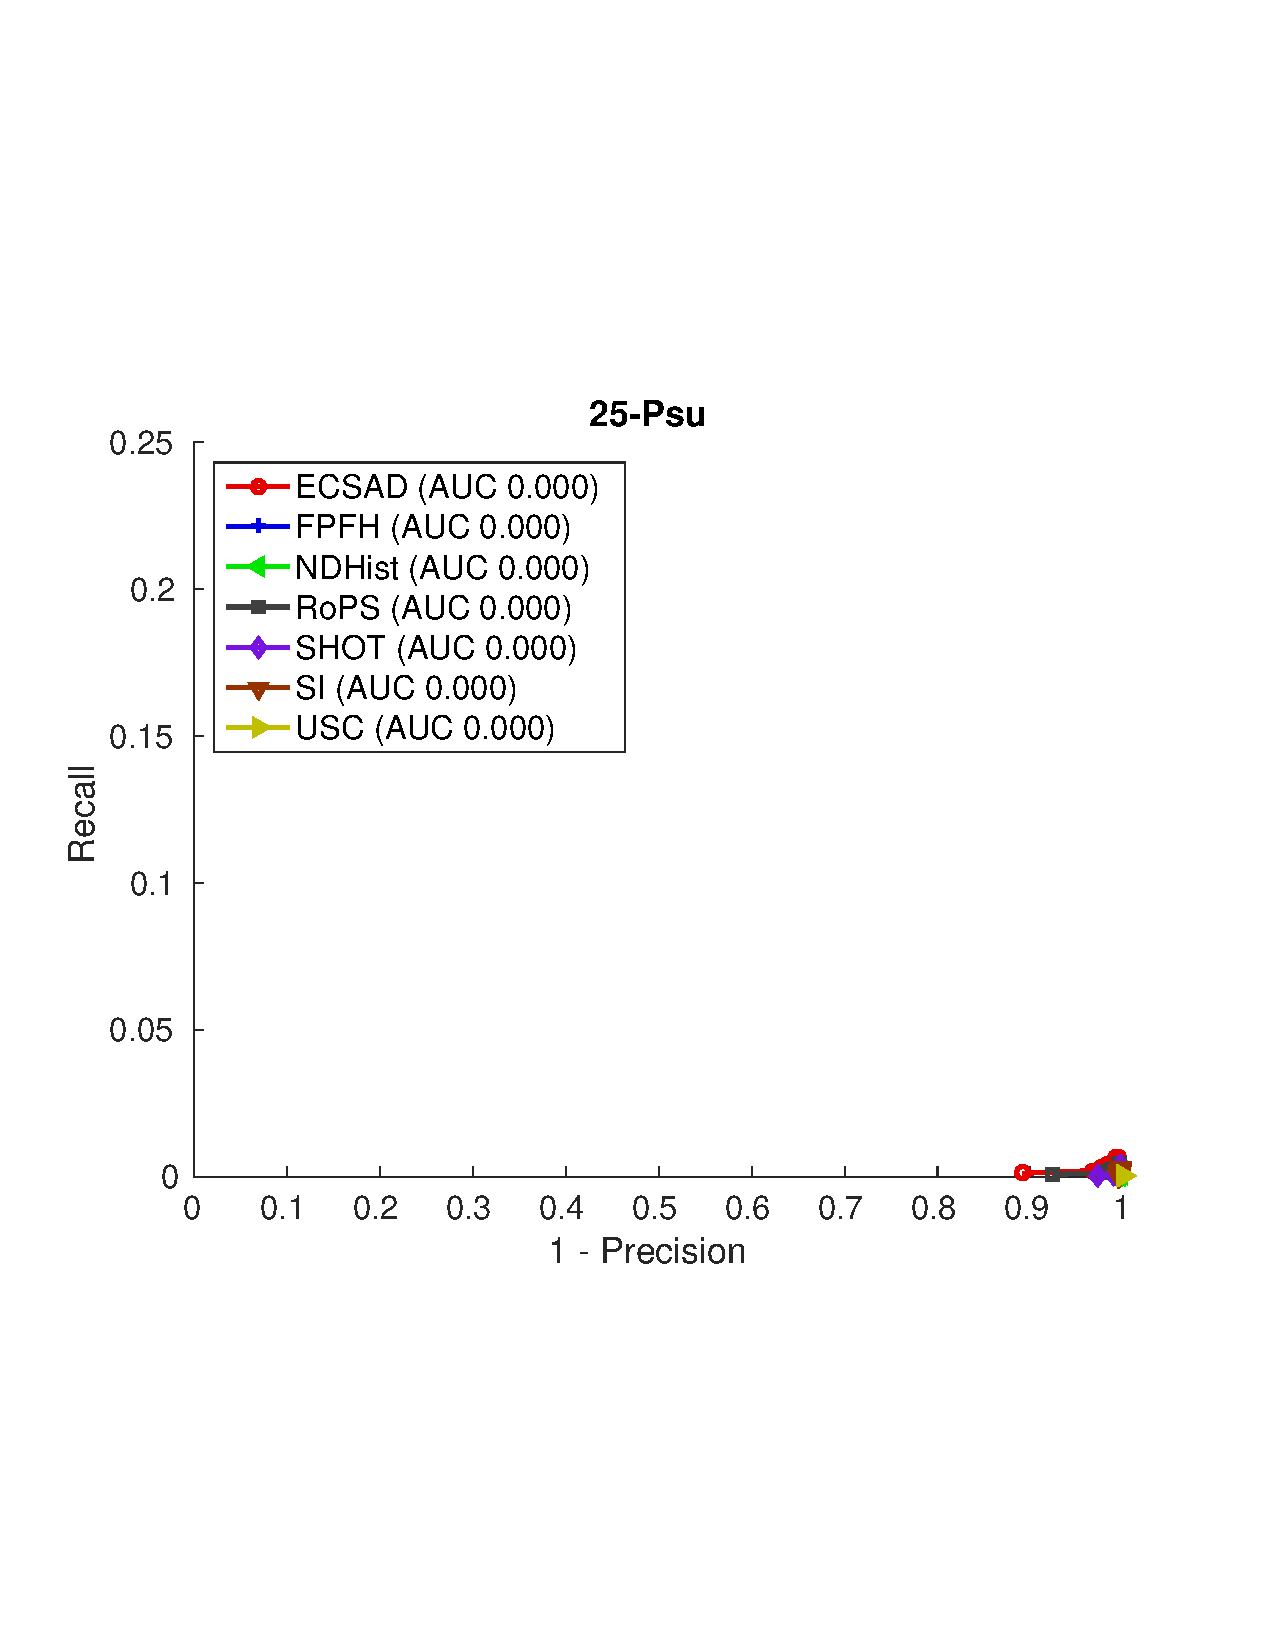
\includegraphics[clip, trim=0.7cm 6cm 0.7cm 6cm,width=1.0\linewidth, height= 1.0\linewidth, keepaspectratio]{img/25-Psu_L2_RATIO_zoom.pdf}
\caption{PRC curve: Psu}\label{fig:noise}
\end{minipage}
\end{figure*}
  
%\textbf{Gr. 1}  &\textbf{Gr. 2} &\textbf{Gr. 3} p{0.8cm} p{0.8cm} p{0.8cm}



%-------------------------------------------------------------------------
\clearpage
{\small
\bibliographystyle{3dv2016authorkit/latex/ieee}
\bibliography{bib}
}

\end{document}
